\documentclass{IEEEtran}
\IEEEoverridecommandlockouts
\usepackage{cite}
\usepackage{amsmath,amssymb,amsfonts}
\usepackage{algorithmic}
\usepackage{graphicx}
\usepackage{textcomp}
\usepackage{xcolor}
\usepackage{datetime}
\def\BibTeX{{\rm B\kern-.05em{\sc i\kern-.025em b}\kern-.08em
    T\kern-.1667em\lower.7ex\hbox{E}\kern-.125emX}}
\usepackage{hyperref}
\usepackage{booktabs}
\usepackage{dsfont}
\usepackage{tablefootnote}
\usepackage{float}
\usepackage[justification=centering]{caption}

\DeclareMathOperator*{\argmax}{arg\,max}
\DeclareMathOperator*{\argmin}{arg\,min}
\graphicspath{{img/}}

% \title{Optimizing Aircraft Engine RUL Prediction with Bayesian-Enhanced Interpretable ML and SHAP}
\title{Enhancing Aircraft Engine RUL Prediction: Interpretable Models and Bayesian Optimization}

\author{\IEEEauthorblockN{
    Juan Echeagaray \IEEEauthorrefmark{1},
    Jonathan Montalvo-Urquizo \IEEEauthorrefmark{2} and
    María Guadalupe Villarreal-Marroquín \IEEEauthorrefmark{3}\\}
\IEEEauthorblockA{
    School of Engineering and Sciences \\
    Tecnologico de Monterrey\\
    Monterrey, Nuevo León, México\\
Email: \IEEEauthorrefmark{1}\href{mailto:pabloechg@outlook.com}{pabloechg@outlook.com},
\IEEEauthorrefmark{2}\href{mailto:jmontalvo@tec.mx}{jmontalvo@tec.mx},
\IEEEauthorrefmark{3}\href{mailto:maria.villarreal@tec.mx}{maria.villarreal@tec.mx}}}

% \author{\IEEEauthorblockN{Juan Echeagaray}
% \IEEEauthorblockA{
%     School of Engineering and Sciences \\
%     Tecnologico de Monterrey\\
%     Monterrey, Nuevo León, México\\
% Email: \href{mailto:pabloechg@outlook.com}{pabloechg@outlook.com}}}


\begin{document}
    \maketitle

    \begin{abstract}
        This project aims to develop an advanced predictive maintenance (PdM) framework for turbofan engines, a crucial component of aircraft operation. Predicting Remaining Useful Life (RUL) is essential for maintaining safety and efficiency. The approach involves converting run-to-failure data into more efficient formats, segmenting flights, and extracting features using statistical descriptors. A variety of efficient machine learning models are employed, with the selected model predicting RUL, while Bayesian Optimization is applied to optimize this primary model and the two secondary models that provide the prediction intervals. Interpretability is ensured using Shapley values.

        Efficiency is demonstrated through a proof of concept using the NCMAPSS dataset, showing that accurate RUL estimates can be achieved on a personal computer with a standard GPU. Performance is expected to improve when implemented on dedicated hardware. This framework is anticipated to significantly reduce operational costs by enabling informed maintenance scheduling, thereby enhancing safety and reliability.
    \end{abstract}
    \begin{IEEEkeywords}
        Predictive Maintenance, Time Series Segmentation, XGBoost, SHAP, Prediction Intervals, Bayesian Optimization.
    \end{IEEEkeywords}

    \section{Introduction}

        Modern industries heavily rely on condition-based monitoring systems to collect and analyze vast amounts of data from machinery, encompassing sensor readings, vibrations, temperatures, acoustic data, and more \cite{Azari2023}, \cite{Achouch2022}. These data serve as the backbone for assessing the Remaining Useful Life (RUL) of critical equipment. Accurate RUL predictions hold immense significance, as they offer the potential to revolutionize operational efficiency by enabling preventive maintenance precisely when required. This approach not only reduces maintenance costs \cite{brink-2021} but also enhances the sustainability of organizations \cite{karuppiah2021sustainable} and provides a competitive edge over industry counterparts. Moreover, in safety-critical scenarios, such as aviation (where turbofan engines play a pivotal role), precise RUL predictions are crucial to avoid catastrophic mid-flight engine failures and production line stoppages.

        From a computational perspective, three primary modeling approaches have emerged: physics-driven models, data-driven models, and hybrid models that combine aspects of both. Among these, data-driven models have gained prominence due to their relatively straightforward implementation and remarkable accuracy. This category, particularly, has been dominated by the application of deep learning techniques, which are adept at capturing intricate relationships within the data collected from Condition-Based Monitoring (CBM) systems \cite{data-driven-survey}, \cite{phm2021-1st-cnn}, \cite{phm2021-2nd-inception}, \cite{phm2021-3rd-stacked-cnn}, \cite{pi-dl-rul}. However, the computational demands associated with training and deploying deep learning models often pose challenges, making them unsuitable for certain scenarios. In such cases, lower-footprint models like gradient boosting algorithms and linear models may offer a more practical alternative, albeit with slightly reduced performance. These models also lend themselves well to hyperparameter tuning, which can be difficult to achieve with most deep learning approaches.

        While a significant portion of research endeavors is focused on enhancing model performance, an equally crucial but often neglected aspect is model interpretability. In the current landscape of machine learning and AI, model interpretability and accountability hold paramount importance. These qualities are not just regulatory requirements; they are markers of responsible AI development. Laws such as the General Data Protection Regulation (GDPR) \cite{gdpr-act} and the Algorithmic Accountability Act \cite{govinfo-2022} have reinforced the necessity for algorithms deployed to the general public to be transparent and accountable.

        Beyond compliance, these laws underscore the fundamental principle that a trustworthy AI model should not only make accurate predictions but also provide insights into why it arrives at those conclusions. This ensures that AI systems are transparent, understandable, and ultimately serve as valuable tools in an ever-evolving technological ecosystem. As a new trend gains momentum, placing model interpretability on the same level as model accuracy, it reinforces the idea that model transparency and accountability are essential for ethical and reliable AI systems. The main question is not so much if we can get an explainable AI (XAI) solution, but rather if it we can get an XAI with an accuracy comparable to that of regular AI/ML? \cite{angelov2021explainable}

        In the broader field of machine learning, Shapley values have been extensively used to improve model understanding. For example, \cite{shap-health} demonstrated the utility of Shapley values in understanding the contributions of auxiliary inputs such as sex and age for accurate detection of acute myocardial infarction. Furthermore, the work by \cite{shap-credit-lending} emphasized how Shapley values can help accurate ML models become transparent in critical scenarios such as Peer-to-Peer lending. In the context of predictive maintenance (PdM), it becomes imperative to establish means for comprehending and explaining model predictions, making the insights from these studies highly relevant to this domain.

        In line with model interpretation, the issue of prediction uncertainty is crucial. Studies across various domains have highlighted the importance of incorporating prediction intervals (PI) in machine learning models \cite{pi-motivation}. For instance, in stock forecasting, PI application builds trust in risk analysis models \cite{pi-stock}. Similarly, in wind power production, PI aids in understanding future energy yield for reliability and cost-effectiveness \cite{pi-wind-power}. Moreover, in predicting Remaining Useful Life (RUL) of engines, PI helps schedule maintenance accurately \cite{pi-dl-rul}.

        Integrating prediction intervals provides stakeholders valuable insights into prediction ranges or confidence levels. This additional information facilitates informed decision-making, balancing maintenance needs and operational efficiency.

        The paper is organized as follows: Section \ref{sec:problem_statement} formally introduces the problem to be addressed, while Section \ref{sec:objectives} outlines the research objectives and the corresponding evaluation metrics used to assess performance. In Section \ref{sec:methodology}, the quantitative techniques to be used are introduced. Finally, Sections \ref{sec:results} and \ref{sec:conclusion} present the main findings and conclusions, as well as directions for future research.

    \section{Problem Statement} \label{sec:problem_statement}

        The foundation for this work is the New Commercial Modular Aero-Propulsion System Simulation (NCMAPSS) dataset proposed in \cite{ncmapss-dataset}, encompassing sensor readings, environmental descriptors, auxiliary variables, virtual sensor readings, and RUL values; the NCMAPSS dataset represents an upgrade from the previous CMAPSS dataset by the inclusion of real world flight conditions into the simulation regime. Figure \ref{fig:turbofan_diagram} aids in conceptualizing the core components of a turbofan engine, as represented in the NCMAPSS dataset \cite{ncmapss-dataset}.
        \begin{figure}[!htbp]
            \centering
            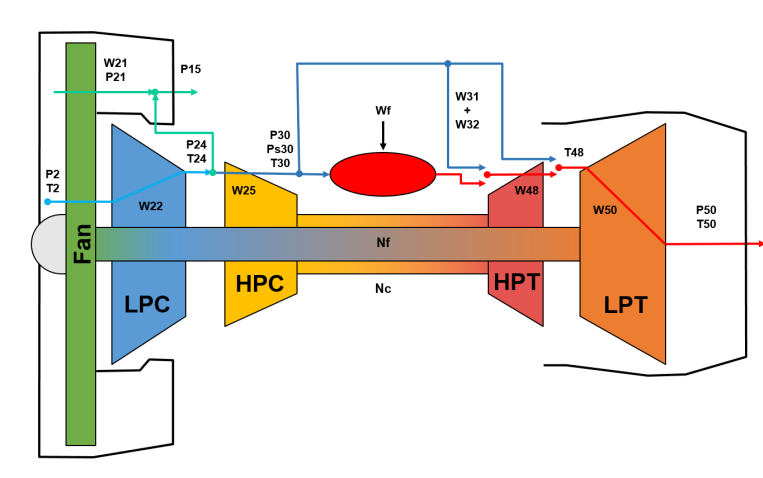
\includegraphics[width=0.95\columnwidth]{cmapss_turbofan.png}
            \caption{NCMAPSS Turbofan engine diagram, taken from \cite{ncmapss-dataset}.}
            \label{fig:turbofan_diagram}
        \end{figure}

        The NCMAPSS dataset, distinguished by its high quality, served as the chosen data source for the PHMAP 2021 Data Challenge \cite{chao2021phm}. It was prioritized over the CMAPSS dataset due to its incorporation of a broader range of flying conditions and multiple failure modes, providing a more realistic simulation of actual flights with heightened fidelity. While sharing the fundamental objective with PHMAP of estimating the remaining useful life (RUL) for a fleet of turbofan engines under challenging conditions, the current research extends this aim by applying more stringent constraints:

        \begin{itemize}
            \item \textbf{Efficient Modeling:} Given computational limitations, the chosen model for training must prioritize efficiency. This constraint rules out most deep learning approaches, which may be computationally intensive.
            \item \textbf{Model Interpretability:} In light of the criticality of the situation, model interpretability is paramount. It is imperative to understand why a model produces a specific RUL estimate, ensuring transparency and trustworthiness of the predictions.
            \item \textbf{Confidence and Prediction Intervals:} Additionally, there is a need to develop confidence in the model's predictions. This entails providing prediction intervals for each RUL estimate, allowing for a better assessment of the prediction's reliability.
        \end{itemize}

    \section{Objectives} \label{sec:objectives}

        The primary objectives of this study are to develop:
        \begin{enumerate}
            \item PdM framework to predict RUL for a designated fleet of machinery.
            \item Models which ensure reproducibility, stability, robustness and confidence.
            \item Tools to interpret and visualize the model's predictions.
        \end{enumerate}

        The previous objectives are to be accomplished subject to the following constraints and assumptions:
        \begin{itemize}
            \item RUL prediction of an uniform fleet of machines.
            \item Availability of a labeled dataset with run to failure sequences of each machine.
        \end{itemize}

        \subsection{Evaluation Metrics}

            This paper follows the metric definitions for \eqref{eqn:phmap_loss} in \cite{ncmapss-dataset} to develop comparable results with prior research. Given two vectors $y, \hat{y} \in \mathbb{R}^{m}$ representing real RUL labels and RUL estimates (unscaled), the PHMAP loss function for the predictive model is defined as:

            \begin{equation} \label{eqn:phmap_loss}
                \begin{gathered}
                    \text{RMSE}(y, \hat{y}) = \sqrt{\frac{1}{m}\sum_{i=1}^{m} (y_i - \hat{y}_i)^{2}} \\
                    \textit{NASA}(y, \hat{y}) = \frac{1}{m}\sum_{i=1}^{m} \left[\exp (\alpha \cdot (y_i - \hat{y}_i)) - 1\right]\\
                    \alpha = \begin{cases}
                        \frac{-1}{10} & \text{if } y_i - \hat{y}_i \leq 0 \\
                        \frac{1}{13} & \text{if } y_i - \hat{y}_i > 0
                    \end{cases}  \\
                    \mathcal{L}(y, \hat{y}) = \frac{1}{2} \left(\text{RMSE}(y, \hat{y}) + \textit{NASA}(y, \hat{y})\right). \\
                \end{gathered}
            \end{equation}

            NASA's scoring function is popularly used in aeronautics since it is an asymmetric loss function with higher penalties for overestimates \cite{saxena2008damage}.

            In addition to RUL point estimates, this research also aims to develop a model for estimating prediction intervals for any RUL prediction; the loss function to optimize being the Mean Pinball Loss subject to a specified quantile $\tau$, defined as
            \begin{equation}\label{eqn:pinball}
                \begin{gathered}
                    \beta = \begin{cases}
                        \tau & \text{if } y_i - \hat{y}_i \geq 0 \\
                        \tau - 1 & \text{if } y_i - \hat{y}_i < 0
                    \end{cases}  \\
                    \mathcal{L}_\tau(y, \hat{y}) = \frac{1}{m} \sum_{i=1}^{m} \beta (y_i - \hat{y}_i).
                \end{gathered}
            \end{equation}

    \section{Quantitative Techniques} \label{sec:methodology}

        In this section, the quantitative techniques employed in the study are outlined. For a visual overview of the process, the diagram in Figure \ref{fig:methodology_diagram} provides a comprehensive overview of the research methodology, depicting the step-by-step process flow employed in this study.
        \begin{figure*}[!htbp]
            \centering
            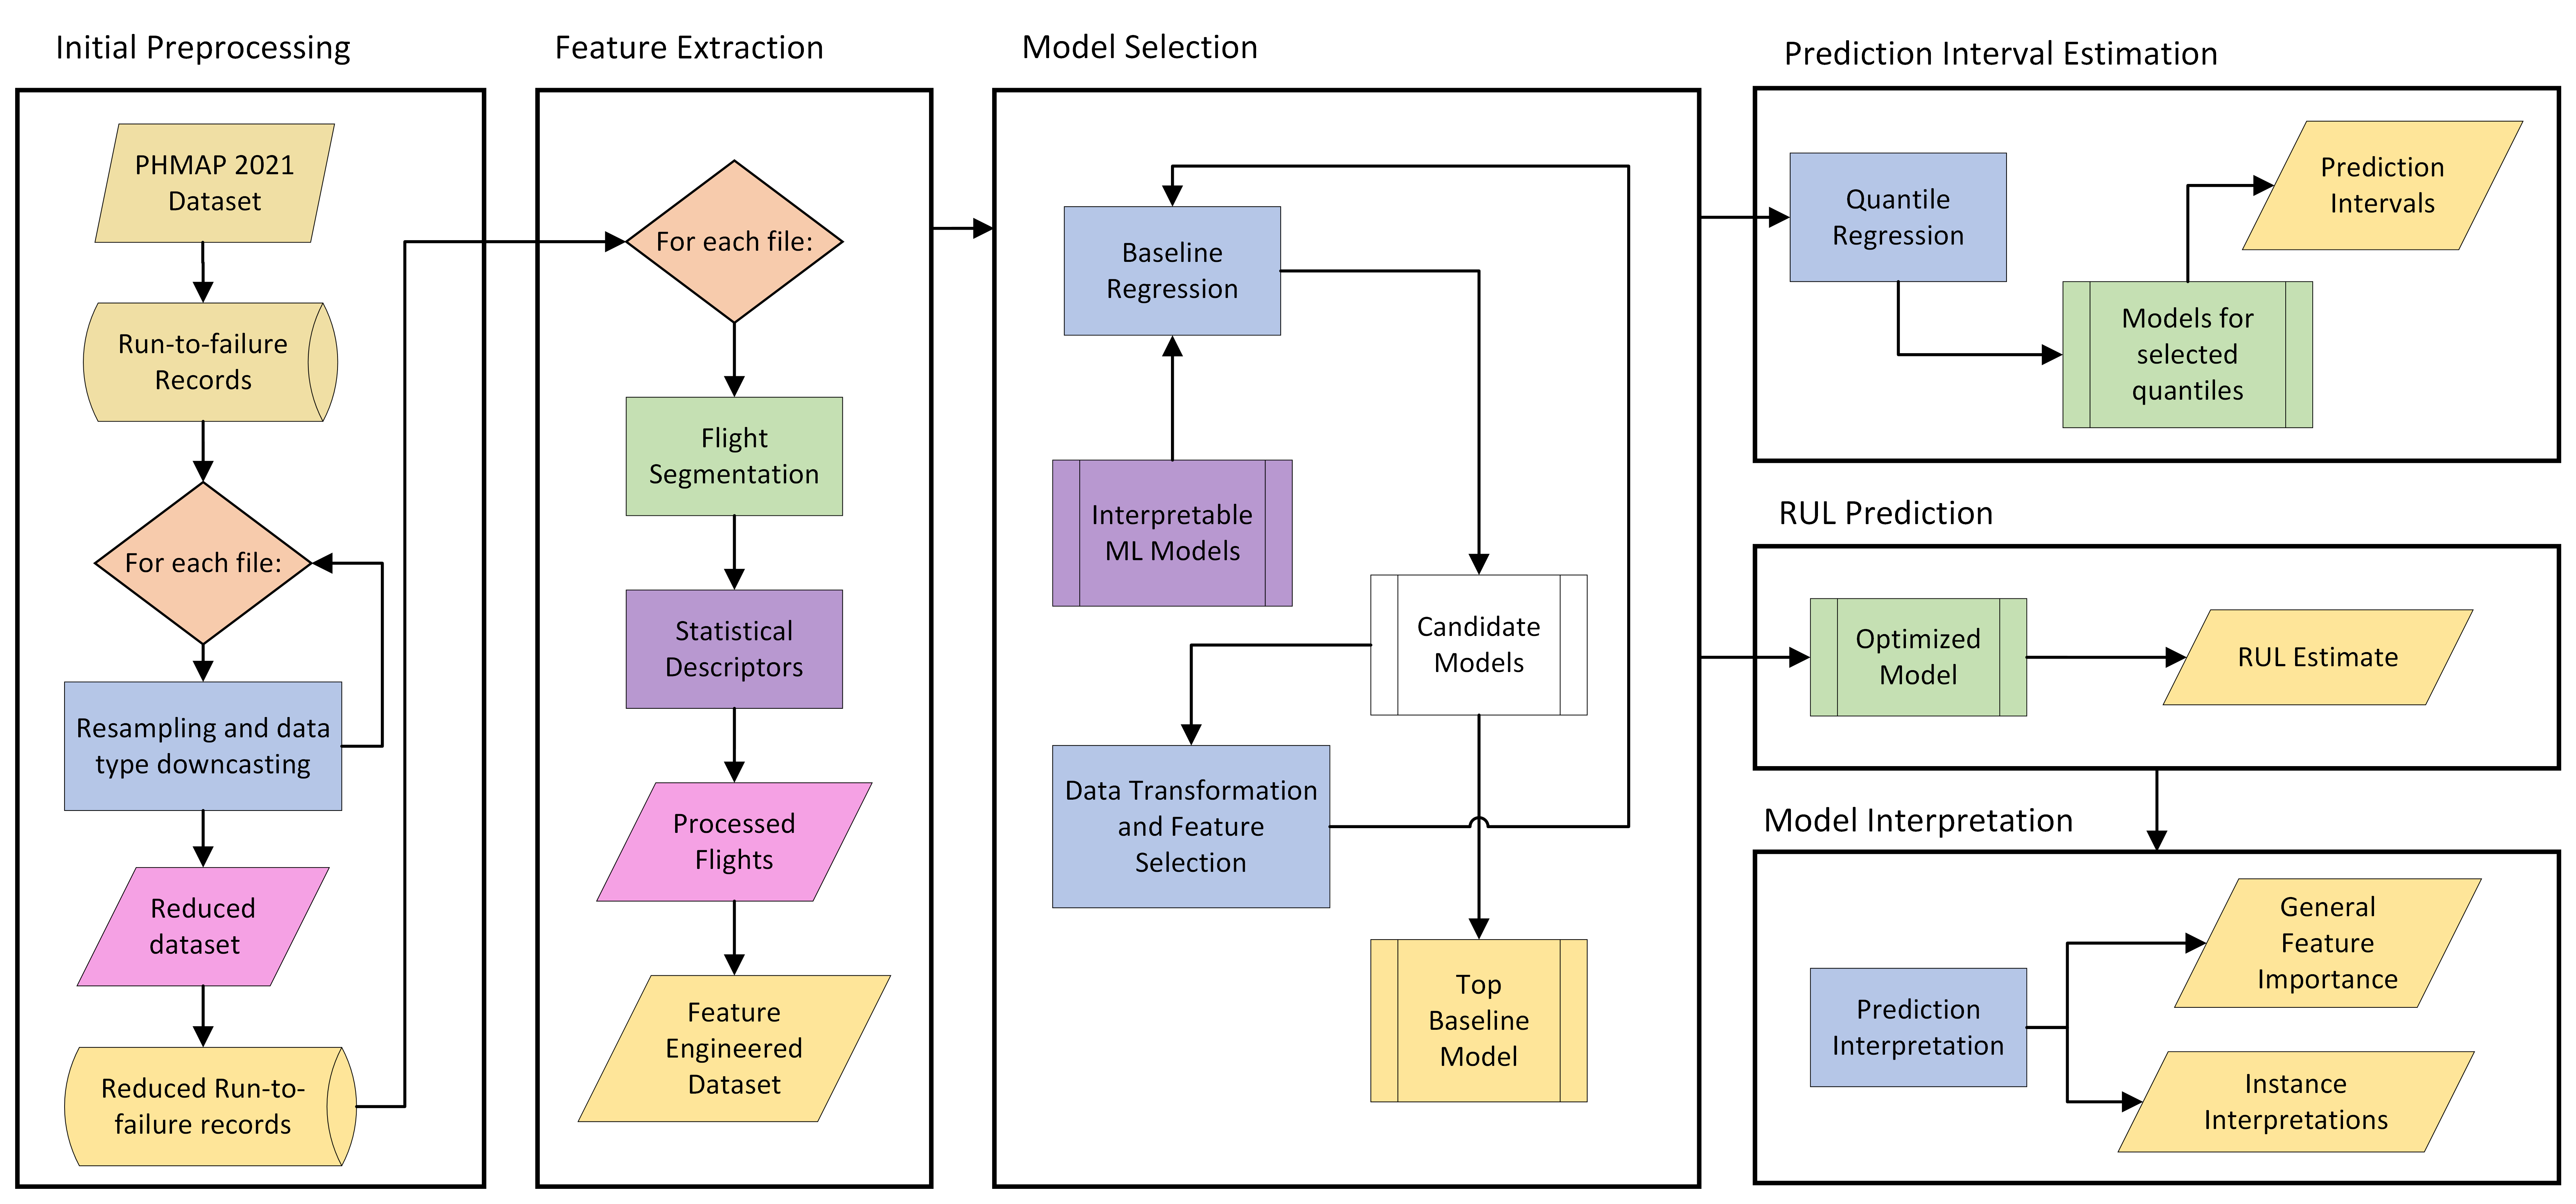
\includegraphics[scale=0.27]{research_diagram.png}
            \caption{Proposed methodology overview.}
            \label{fig:methodology_diagram}
        \end{figure*}

        \subsection{Data Resampling and Downcasting} \label{sec:resampling}

            In dealing with large datasets that exceed the capacity of a personal computer's memory, practical solutions are essential for efficient iterative research. One such approach involves resampling the data, typically recorded over several hours, to a coarser granularity, such as every $n$ seconds (see Figure \ref{fig:resampling}). This step significantly reduces the computational load while preserving the core information needed for analysis.
            \begin{figure}[!htbp]
                \centering
                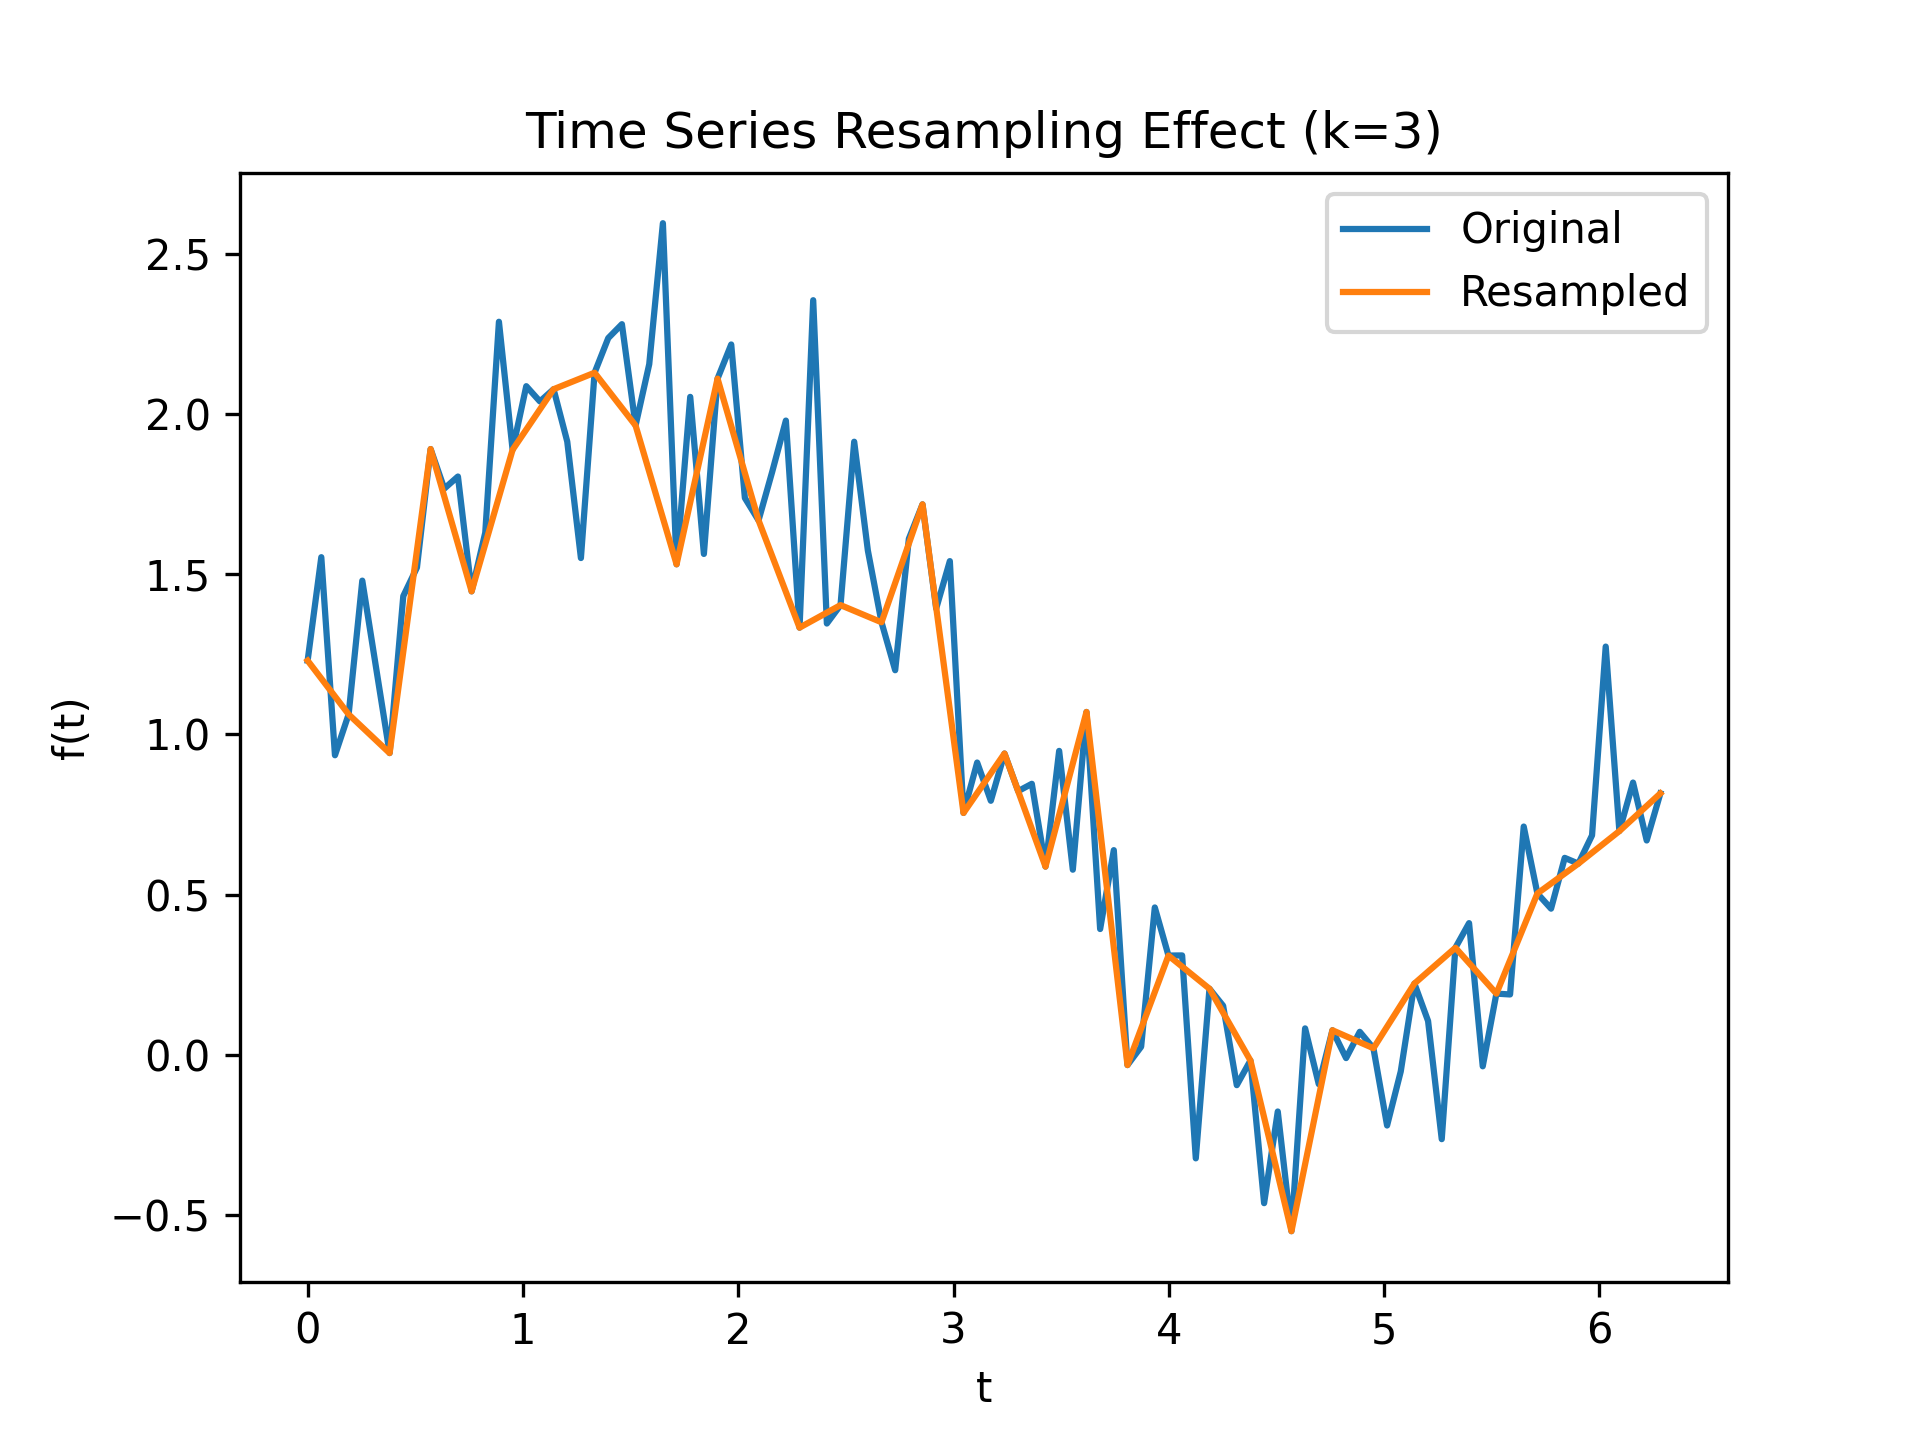
\includegraphics[scale=0.45]{resampling_series.png}
                \caption{Example of time series resampling (keep every $k$th record).}
                \label{fig:resampling}
            \end{figure}

            Additionally, downcasting data types from 64-bit floating points to 32-bit floating points proves valuable in optimizing computational resources. Although 64-bit precision is often more than necessary for many analysis tasks, it comes at a cost in terms of computational complexity and memory usage. Downcasting to 32-bit floating points minimizes these issues without substantially compromising the integrity of the analysis. In most cases, the loss of precision is negligible.

            Furthermore, Table \ref{tab:raw_sizes} provides an overview of the dataset sizes used in this work, highlighting the impact of these strategies on data manageability.
            \begin{table}[!htbp]
                \caption{Size of each dataset in the PHMAP 2021 Competition (in GB).}
                \label{tab:raw_sizes}
                \centering
                \begin{tabular}{ll}
                    \toprule
                    Dataset & Size (GB) \\
                    \midrule
                    DS01-005.h5 & 2.9 \\
                    DS02-006.h5 & 2.5 \\
                    DS03-012.h & 3.7 \\
                    DS04.h5 & 3.8 \\
                    DS05.h5 & 2.6 \\
                    DS06.h5 & 2.5 \\
                    DS07.h5 & 2.7 \\
                    DS08a-009.h5 & 3.2 \\
                    DS08c-008.h5 & 2.4 \\
                    DS08d-010.h5 & 2.9 \\
                    DS\_Validation\_f.h5 & 2.9 \\
                    \midrule
                    Total & 32.1 \\
                    \bottomrule
                \end{tabular}
            \end{table}

            Implementing these strategies (data resampling and datatype downcasting) not only eases data handling in resource-constrained settings but also ensures that critical information remains intact, facilitating streamlined and efficient iterative studies.

        \subsection{Time Series Segmentation} \label{sec:segmentation}

            Machine learning models often require fixed-shaped individual samples, making segmentation critical. It is hypothesized that valuable time series information resides within its segments. By emphasizing segmentation and feature extraction at this level, we aim to create a richer dataset for training machine learning models.

            \subsubsection{Feature Scaling}

                Given the distinct scales of the variables present in the dataset, a Min-Max scaling routine \eqref{eqn:min_max} is applied on each flight individually. For any given flight encoded in a matrix $X \in \mathcal{M}_{d}^{T}(\mathbb{R})$, of $T$ rows (i.e., flight length) and $d$ columns (i.e., number of sensors):
                \begin{equation} \label{eqn:min_max}
                    \begin{gathered}
                        X_{min} = \mathds{1}_{(d \times 1)} \min_i \{m_{ij}: 1 \leq i \leq T, \forall j \in \{1, \dots d\}\} \\
                        X_{max} = \mathds{1}_{(d \times 1)} \max_i \{m_{ij}: 1 \leq i \leq T, \forall j \in \{1, \dots d\}\} \\
                        X_{std} = \frac{(X - X_{min})}{X_{max} - X_{min}}.
                    \end{gathered}
                \end{equation}

            \subsubsection{Binary Segmentation}

                In dealing with extensive flight data processing, the use of approximate methods for time series segmentation proves to be essential. This section explores these efficient techniques, chosen to manage the sheer volume of flight records. These methods have shown promising results, making them a practical choice for large-scale time series analysis.

                For a given signal $Y = \{y_t\}_{t=1}^{t=T}$ of $T$ samples, where $y_t \in \mathbb{R}^d$, we assume there exists a set $\mathcal{T} = \{t_{1}^{*}, t_{2}^{*}, \dots, t_{n}^{*}\}$ coding the $n-1$ stages of $Y$. As an example, see the time series depicted in Figure \ref{fig:changepoint_example}, the real set $\mathcal{T}$ for this series would be $\{158, 332, 500\}$.
                \begin{figure}[!htbp]
                    \centering
                    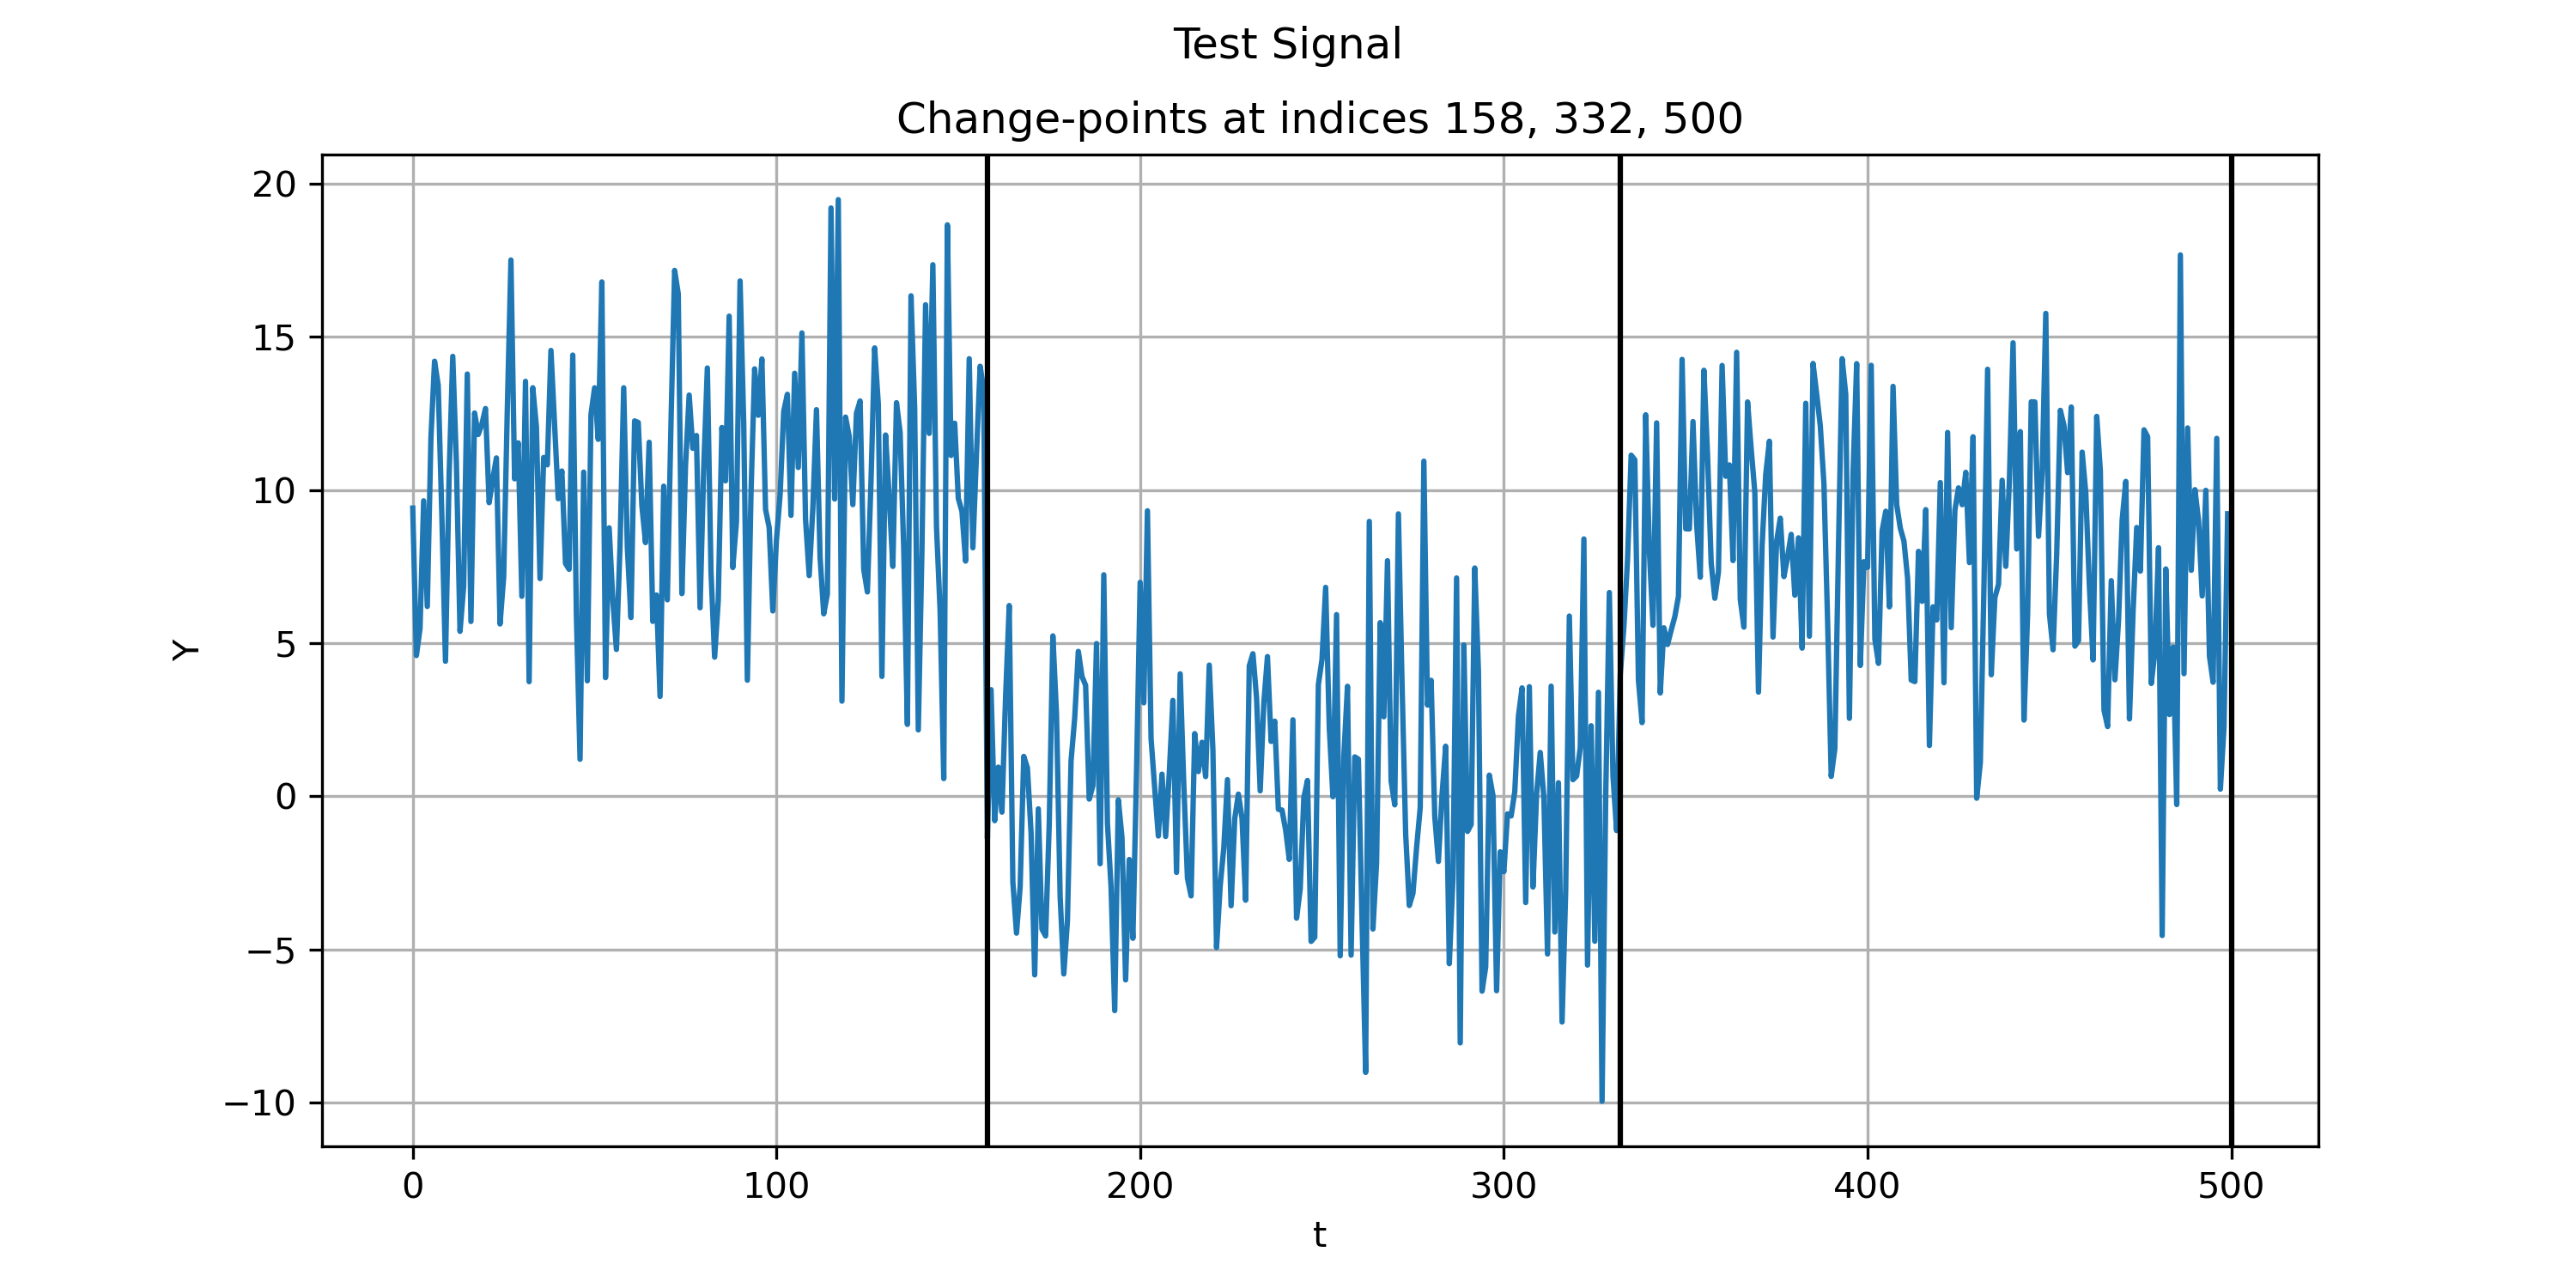
\includegraphics[scale=0.36]{show_series.png}
                    \caption{Example of change points in univariate time series.}
                    \label{fig:changepoint_example}
                \end{figure}

                Change point detection consists in searching for the optimal segmentation $\mathcal{T}$ of a time series $y$ \cite{truong2020selective}. An easy approach to establish a loss function for the algorithm is to simply define such loss as \eqref{eqn:change_loss} where $C$ is a measure of the goodness of fit for the selected signal:
                \begin{equation}\label{eqn:change_loss}
                    V(\mathcal{T}, y) = \sum_{k=0}^{K} C(y_{t_k, t_{k+1}}).
                \end{equation}

                A popular choice for $C$ is the L2 loss, given a subset $y_\mathcal{I} = \left\{y_t\right\}_{t \in \mathcal{I}}$ and $\bar{y}$ being the component wise mean of $y_{\mathcal{I}}$, the L2 loss is defined as:
                \begin{equation}\label{eqn:l2_segment_loss}
                    C(y_{\mathcal{I}}) = \sum_{d} \sum_{t \in \mathcal{I}} ||y_t - \bar{y} ||_{2}^{2}.
                \end{equation}

                Binary Segmentation is an approximate method to estimate the real set $\mathcal{T}$, it's a sequential greedy algorithm \cite{truong2020selective}, \cite{jiang2023time} that estimates the first change point as described in:
                \begin{equation} \label{eqn:binseg}
                    \hat{t}_{1} := \argmin_{1 \leq t < T - 1} C(y_{0 \dots t}) + C(y_{t \dots T}).
                \end{equation}

                Binary Segmentation may also be constrained to a subset of possible change points by fixing some external hyperparameters, such as the minimal size for a segment and the indices at which segment splits are tested. The present study empirically chose a minimum size of $\lfloor 0.12 \cdot T\rfloor$ and a restriction on the indices to be of the form $\lfloor 0.05 \cdot T \rfloor$. These parameters may be subject to the hyperparameter optimization regime proposed in Section \ref{sec:hyperparameter}, but its left out due to time and resource constraints.

            \subsubsection{Feature Engineering}

                The uniform segments obtained from the previous segmentation step serve as the foundation for feature engineering. In this section, a set of statistical descriptors is applied to each of these segments, generating a feature vector that encapsulates all relevant information from a flight.

                Given a segment $S_{i}$ from a sample $F$, which encompasses $T_i$ timestamps, $S_i \in \mathcal{M}_{d}^{T_i}(\mathbb{R})$ with $T_i \geq \alpha$ where $\alpha$ is a constraint on the minimum size of $S_i$. A set of descriptors $\mathcal{F}_s = \{f \mid  f: \mathcal{M}_{d}^{T_i}(\mathbb{R}) \rightarrow \mathbb{R}^{d}\}$ is applied on each segment $S_i$ individually, this research employs the descriptors in Table \ref{tab:stat_descriptors}:
                \begin{table}[!htbp]
                    \centering
                    \caption{Proposed set of statistical descriptors.}
                    \label{tab:stat_descriptors}
                    \begin{tabular}{ll}
                        \toprule
                        \multicolumn{2}{c}{Statistical Descriptors} \\
                        \midrule
                        Minimum & Std. Deviation \\
                        25th Percentile & Variance \\
                        Median & Kurtosis \\
                        75th percentile & Skew \\
                        Maximum & Coefficient of Variation \\
                        Mean & - \\
                        \bottomrule
                    \end{tabular}
                \end{table}

                Applying each statistical descriptor on all the segments $S_i$, results in a feature vector $\hat{F} \in \mathbb{R}^{d \cdot |\mathcal{F}_s| \cdot |S| }$. Given the frequent calls to these statistical descriptor functions, prioritizing efficient implementations is essential to streamline computational resources for timely analysis.

                In cases where the resulting vector exhibits high dimensionality, it may be beneficial to apply a feature selection algorithm; a simple approach would be to select features based upon a variance threshold under the assumption that nearly constant features offer little value to a machine learning model \cite{li2017feature}. The choice of threshold is arbitrary and should be part of any hyperparameter optimization regime.

        \subsection{Model Selection} \label{sec:model}

            In the model selection phase, we start with a processed dataset and create an 80-20 train-test split for robust evaluation. We then choose efficient machine learning models (see Table \ref{tab:interpretable_models} for the proposed list) with characteristics such as linear regression coefficients or decision tree splits. These models are fitted and evaluated on both training and test subsets \footnote{Mean Squared Error is chosen as a common loss function to optimize}, calculating PHMAP loss and RMSE for each and recording total training times.
            \begin{table}[!htbp]
                \centering
                \caption{Proposed set of ML models.}
                \label{tab:interpretable_models}
                \begin{tabular}{ll}
                    \toprule
                    \multicolumn{2}{c}{Interpretable Models} \\
                    \midrule
                    Linear Regression \cite{scikit-learn} & Ridge Regression \cite{scikit-learn}\\
                    Lasso \cite{scikit-learn} & LassoLars \cite{scikit-learn} \\
                    ElasticNet \cite{scikit-learn} & Random Forest \cite{scikit-learn} \\
                    XGBoost \cite{xgboost} & LightGBM \cite{ke2017lightgbm} \\
                    Catboost \cite{catboost} & SVM \cite{scikit-learn} \\
                    Decision Tree \cite{scikit-learn}& Dummy Regression (Mean) \cite{scikit-learn} \\
                    \bottomrule
                \end{tabular}
            \end{table}

            If necessary, apply any data transformation techniques like standardization, scaling, or PCA to improve model performance. This iterative process of model fitting, evaluation, and possible transformation continues until a satisfactory collective performance is achieved.

            After completing the iterations, models are strategically selected based on training scores while taking into account their respective training times. This approach ensures that the chosen algorithms are not only effective but also computationally feasible for subsequent hyperparameter optimization.

        \subsection{Model Interpretability} \label{sec:interpretability}

            Shapley values offer a model agnostic approach to post-hoc model interpretation \cite{chen2023algorithms}, where one explains a single prediction given the original input features. Adapting the original Shapley value formula, which traditionally assesses each player's contribution to game outcomes, allows us to quantify the significance of individual feature values in predicting model outcomes. In this context, the initial coalition $S$ of players turns into the coalition of feature values for any instance in which a model generates predictions. Considering a predictive model $\hat{f}$ trained on a set of $p$ features, the Shapley value for any feature $j$ is determined as the weighted average of all marginal contributions that the feature can make, encapsulating its unique impact on the overall predictive outcome:
            \begin{multline}
                \phi_j = \sum_{S \subseteq \{1, \dots p\} - \{j\}} \frac{ |S|! (p - |S| - 1)! }{p!} \times \\
                (val(S \cup \{j\}) - val(S)).
            \end{multline}

            To estimate the contribution of any given coalition of feature values we marginalize the model predictions over all the features not present in the coalition $S$:
            \begin{equation}
                val(S) = \int \hat{f}(x_1, \dots, x_p) d\mathbb{P}_{x \notin S}.
            \end{equation}

            Shapley values also possess vital properties for effective model interpretability:
            \begin{itemize}
                \item \textbf{Efficiency:} feature contributions express how a single prediction deviates from the mean prediction of $\hat{f}$\begin{equation} \label{eq:shap_efficiency}
                    \sum_{j=1}^{p} \phi_j = \hat{f}(x) - \mathbb{E}[\hat{f}(X)].
                \end{equation}
                \item \textbf{Symmetry:} two features have the same Shapley value if and only if their contributions are the same\begin{equation*}
                    \begin{split}
                        val(S \cup \{j\}) & = val(S \cup \{k\}) \quad \forall S \subseteq \{1, \dots, p\} - \{j, k\} \\
                        & \Rightarrow \phi_j = \phi_k.
                    \end{split}
                \end{equation*}
                \item \textbf{Null Feature:} a feature that has no effect on a prediction has a zero Shapley value\begin{equation*}
                    \begin{split}
                        val(S \cup \{j\}) & = val(S) \quad \forall S \subseteq \{1, \dots, p\} \\
                        & \Rightarrow \phi_j = 0.
                    \end{split}
                \end{equation*}
                \item \textbf{Linearity:} the contribution of an ensemble of models is the same as the sum of the contribution of each model in the ensemble\begin{equation*}
                    \phi_j^{f + g} = \phi_j^{f} + \phi_j^{g}.
                \end{equation*}
            \end{itemize}

            Efficient approximations exist, catering to specific model types like linear, tree-based, and deep learning models. These approximations balance accuracy with computational feasibility \cite{chen2023algorithms}, \cite{molnar2020interpretable}, \cite{shap-feature-analysis}, making Shapley values practical for understanding various machine learning models \cite{shap-health}, \cite{shap-credit-lending}, \cite{shap-extra-ml}.

        \subsection{Prediction Intervals} \label{sec:prediction_intervals}

            In predictive modeling, all predictions inherently carry uncertainty due to various factors, such as data noise and model limitations.

            Prediction intervals offer a practical way to quantify this uncertainty. Instead of providing a single point estimate, they define a range within which future values are likely to fall based on observed variables. When paired with a point estimate, prediction intervals indicate the level of uncertainty associated with that prediction, often expressed as a confidence level (e.g., 90\%, 95\%, 99\%) \cite{barron2022probability}.

            Quantile regression is a powerful technique used to create prediction intervals \cite{pi-stock}, \cite{pi-wind-power}, \cite{pi-dl-rul}. For the base case, it involves developing two models, one for the lower and one for the upper bound of the interval. By specifying the desired confidence level, quantile regression captures the spread of potential outcomes effectively \cite{romano2019conformalized}, \cite{pi-motivation}.

            Quantile regression relies on the Pinball Loss \eqref{eqn:pinball} to model the conditional quantiles of the target variable given the covariates. It can be shown that minimizing the Pinball Loss for a given quantile is equivalent to formulating a Conditional Quantile function for a target variable $y$ given some covariates $X$ \cite{koenker2001quantile}:
            \begin{equation}
                \mathcal{Q}_\tau(Y | X) = \argmin_{q(X)} \mathbb{E}[\mathcal{L}_\tau(Y, q(X))].
            \end{equation}

        \subsection{Hyperparameter Optimization} \label{sec:hyperparameter}

            Hyperparameter optimization methods offer a systematic approach to find improved hyperparameter configurations, avoiding the assumption that default settings are ideal or relying on human intuition.

            Efficient computation is a critical concern when optimizing hyperparameters due to the substantial cost associated with evaluating machine learning models. It is imperative to use algorithms that leverage information from previous evaluations to iteratively suggest better configurations. In contrast to Grid Search and Random Search, which explore the hyperparameter space without learning, Bayesian Optimization algorithms consider each past trial to propose more promising configurations.

            Tree-structured Parzen Estimators (TPE) is a practical implementation of Bayesian Optimization \cite{bergstra2011algorithms}. Instead of modeling the distribution of the objective function given hyperparameters $p(y|x)$, it models the distribution of hyperparameters given the objective function. TPE defines:
            \begin{equation}
                p(x|y) = \begin{cases}
                    g(x) & y < y^{*} \\
                    b(x) & y \geq y^{*}
                \end{cases}
            \end{equation}

            The probability density function $g(x)$ is constructed as a mixture of Gaussian distributions fitted to hyperparameter configurations ${x^{(i)}}$ tied so far, where the associated loss function $f(x)$ is below a predefined threshold $y^{*}$. Any points not meeting this criterion are covered by the distribution $b(x)$. TPE dynamically selects a new threshold, which is a predetermined quantile $\gamma$ of the observed losses at each iteration within the optimization process.

            TPE suggests the next hyperparameter configuration by sampling a point from $g(x)$ that maximizes the ratio in \eqref{eqn:tpe_suggestion}. This ratio serves as an approximation for the Expected Improvement function.
            \begin{equation} \label{eqn:tpe_suggestion}
                \begin{gathered}
                    S_g = \left\{x: x \sim g(x)\right\} \\
                    x_s = \argmax_{x \in S_g} \frac{g(x)}{b(x)}
                \end{gathered}
            \end{equation}

    \section{Results} \label{sec:results}

        \subsection{Computational Resources}
            The present research was conducted in a WSL2 virtual machine with the specifications described in Table \ref{tab:resources}:
            \begin{table}[!htbp]
                \centering
                \caption{Computational Resources used.}
                \label{tab:resources}
                \begin{tabular}{cc}
                    \toprule
                    Component & Detail \\
                    \midrule
                    OS & \texttt{Ubuntu 20.04.6 LTS on Windows 10 x86\_64} \\
                    CPU & \texttt{12th Gen Intel i5-12450H (12) @ 2.496GHz} \\
                    GPU & \texttt{NVIDIA GeForce RTX 3060} \\
                    RAM & \texttt{9949MiB} \\
                    \bottomrule
                \end{tabular}
            \end{table}

            The code necessary to replicate and use the developed tools can be accessed via this \href{https://github.com/JuanEcheagaray75/tec_research_predictive_maintenance}{link}.

        \subsection{Experimental Results}

            By resampling every 5 observations and converting 64-bit floats to 32-bit floats as described in Section \ref{sec:resampling}, the PHMAP dataset experienced a substantial 96\% reduction in its total size (see Table \ref{tab:processed_sizes}). The resulting processed data files are subsequently saved as parquet files, preserving the specified data types.
            \begin{table}[!htbp]
                \caption{Size of each dataset before and after resampling and downcasting.}
                \label{tab:processed_sizes}
                \centering
                \begin{tabular}{lll}
                    \toprule
                    Dataset & Original (GB) & Processed Size (MB) \\
                    \midrule
                    DS01-005 & 2.9 & 113 \\
                    DS02-006 & 2.5 & 97 \\
                    DS03-012 & 3.7 & 142 \\
                    DS04 & 3.8 & 146 \\
                    DS05 & 2.6 & 104 \\
                    DS06 & 2.5 & 102 \\
                    DS07 & 2.7 & 108 \\
                    DS08a-009 & 3.2 & 126 \\
                    DS08c-008 & 2.5 & 96 \\
                    \midrule
                    Total & 26.4 GB & 1034 MB \\
                    \bottomrule
                \end{tabular}
            \end{table}

            Following the application of Binary Segmentation as proposed in Section \ref{sec:segmentation}, with a minimum size requirement of 12\% of the total flight length and the identification of 3 change points, an analysis of the dataset was conducted. The statistical descriptors, as outlined in Table \ref{tab:stat_descriptors}, were computed. Figure \ref{fig:var_coeff_sample} illustrates the Coefficient of Variation for a randomly selected aircraft within the dataset over its initial operational life. The diagram shows two main horizontal axis encoding the flight number the plane took and the sequential number of segment being analyzed; given how early the health state of the sampled plane declined (at its 26th cycle) one can hypothesize that the initial spikes in the variation of fuel flow may be an indicator of an action taken by the pilots or a weather condition that damaged the plane's engine.
            \begin{figure}[!htbp]
                \centering
                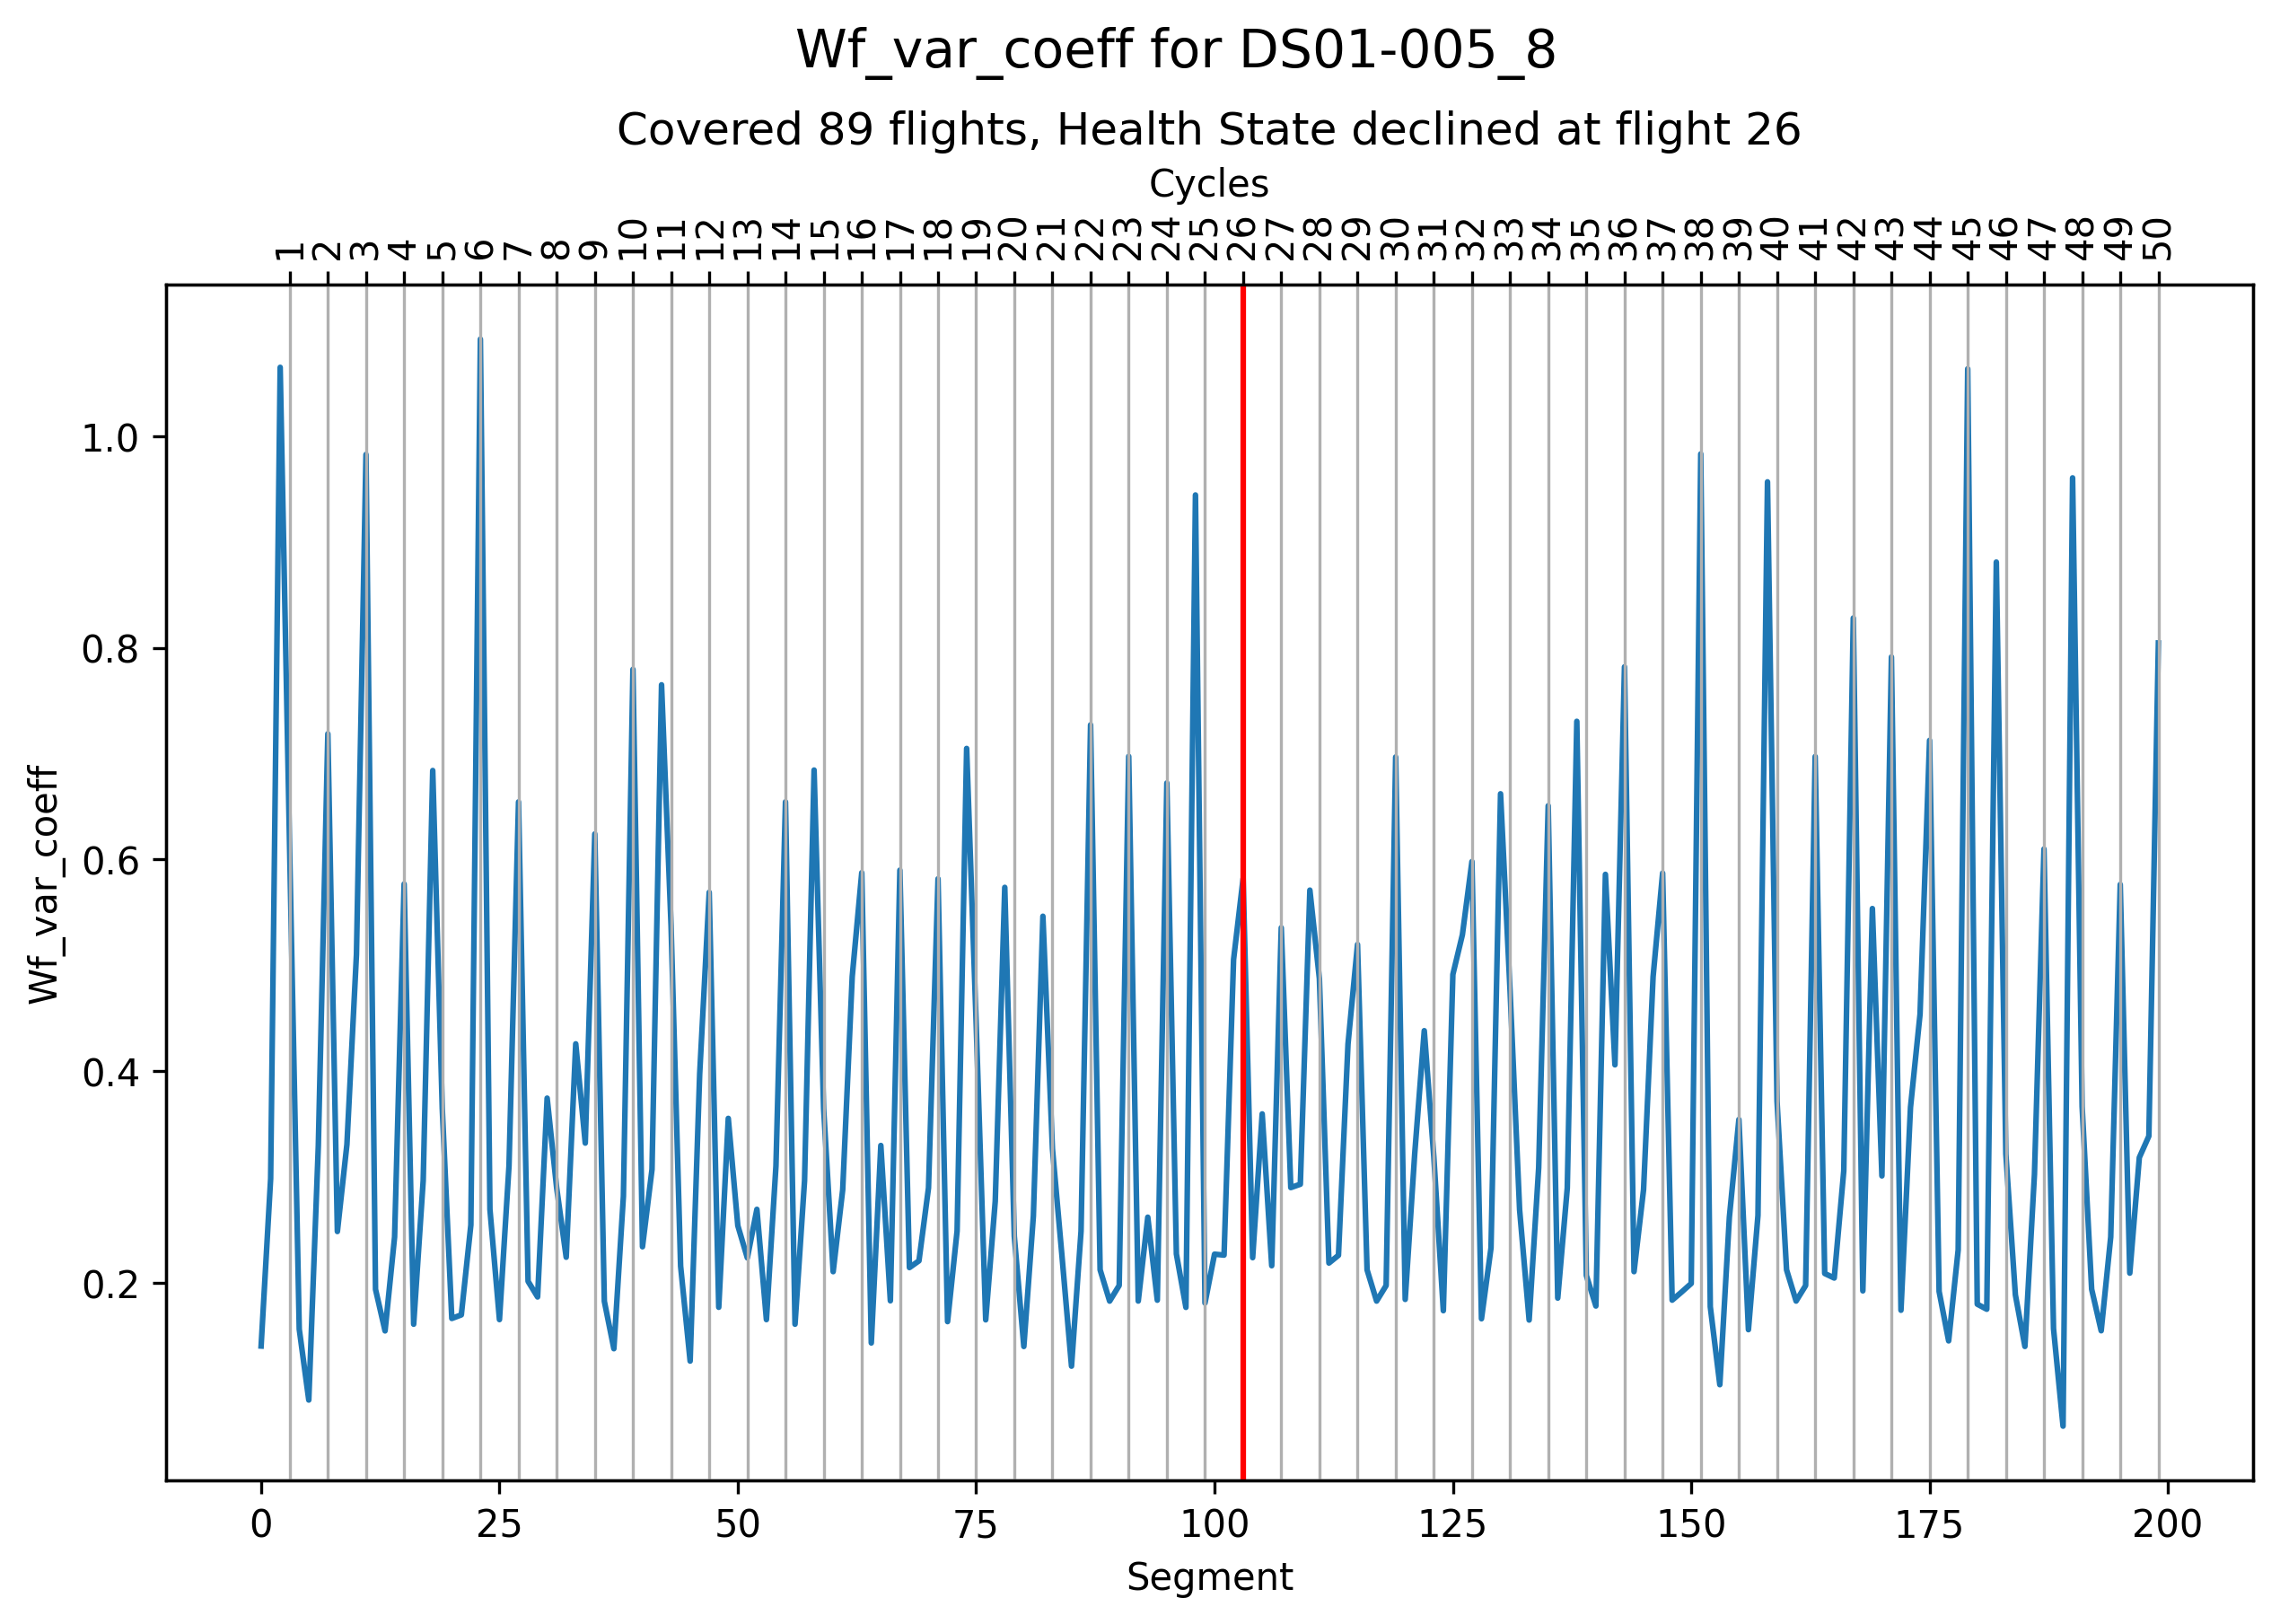
\includegraphics[scale=0.4]{DS01-005_8_Wf_var_coeff.png}
                \caption{Coefficient of Variation for a random plane throughout its operational life.}
                \label{fig:var_coeff_sample}
            \end{figure}

            With the new feature-engineered dataset, the ML models presented in this study underwent training and testing. The dataset was partitioned into an 80-20 split for this purpose, with default hyperparameters used for each model. The models were ranked based on their PHMAP loss on the test set, as indicated in Table \ref{tab:model_scores}. It is noteworthy that models employing the gradient boosting method outperformed other models.
            \begin{table*}[!htbp]
                \centering
                \caption{Train and Test metrics for the selected suite of ML models.}
                \label{tab:model_scores}
                \begin{tabular}{lrrrrr}
                    \toprule
                    Model & Train Loss & Test Loss & Train RMSE (cycles) & Test RMSE (cycles) & Training Time (s) \\
                    \midrule
                    Catboost & 2.043 & 5.321 & 3.769 & 9.399 & 25.692 \\
                    LightGBM & 2.636 & 5.366 & 4.823 & 9.478 & 2.475 \\
                    \textbf{XGBoost} & \textbf{0.697} & \textbf{5.726} & \textbf{1.304} & \textbf{10.048} & \textbf{6.989} \\
                    Random Forest & 2.086 & 5.898 & 3.837 & 10.338 & 223.095 \\
                    Ridge & 6.340 & 6.775 & 11.033 & 11.746 & 0.043 \\
                    Elastic Net & 6.888 & 7.023 & 11.872 & 12.126 & 0.029 \\
                    Lasso & 6.933 & 7.053 & 11.937 & 12.170 & 0.0285 \\
                    Lasso Lars & 6.933 & 7.053 & 11.937 & 12.170 & 0.043 \\
                    SVM & 6.878 & 7.168 & 11.893 & 12.372 & 12.919 \\
                    Decision Tree & 0.0 & 9.472139 & 0.0 & 14.871 & 3.393 \\
                    Dummy (mean) & 16.779 & 17.324 & 23.688 & 24.351 & 0.0008 \\
                    Linear Regression & 5.142 & 87743.231 & 9.112 & 14.664 & 0.246 \\
                    \bottomrule
                \end{tabular}
            \end{table*}

            The recommendation is to use XGBoost, despite not having the lowest loss or the shortest training time among gradient boosting algorithms. This choice is motivated by the maturity of the XGBoost library, its GPU acceleration capabilities (not used for this test), and its widespread use in both research and industry \cite{wind-xgboost}, \cite{pdm-xgboost}, \cite{shwartz2022tabular}, \cite{grinsztajn2022tree}. All these qualities streamline the training and optimization process.

            The TPE algorithm was executed for a total of 500 iterations, serving three distinct models. These models encompass the estimation of the Remaining Useful Life (RUL) of an engine, as well as two additional models responsible for establishing the lower and upper bounds for the prediction interval associated with the RUL estimation.

            Each trial involved a 5-fold cross-validation split, and the result was determined as the average loss over these validation splits. The proposed search space, as well as the best configurations discovered for each model, are detailed in Table \ref{tab:search_space_results}.
            \begin{table}[H]
                \caption{Hyperparameter Search Space for TPE and results for RUL estimators and, Lower and Upper Bounds.}
                \label{tab:search_space_results}
                \centering
                \scalebox{0.95}{
                \begin{tabular}{lrrrr}
                    \toprule
                    Parameter & Range & RUL & Lower & Upper \\
                    \midrule
                    Variance Threshold & $U(0.1, 1)$ & 0.102 & 0.1 & 0.944 \\
                    Learning Rate & $\exp (U(-4.5, 0))$ & 0.021 & 0.116 & 0.042 \\
                    Boosting Rounds & $U_\mathbb{Z}(100, 10000)$ & 1963 & 5859 & 3830 \\
                    Max Depth & $U_\mathbb{Z}(2, 30)$ & 30 & 15 & 20\\
                    Min Child Weight & $U_\mathbb{Z}(2, 50)$ & 29 & 41 & 38 \\
                    Subsample & $U(0.01, 1)$ & 0.726 & 0.854 & 0.795 \\
                    Gamma & $ U(0, 100)$ & 62.667 & 0.124 & 0.109 \\
                    Alpha & $ U(0, 100)$ & 8.721 & 18.859 & 11.387 \\
                    Lambda & $ U(0, 100)$ & 34.832 & 20.921 & 82.706\\
                    \midrule
                    Loss & - & 5.687 & 1.853 & 2.399 \\
                    \bottomrule
                \end{tabular}}
            \end{table}

            In Figure \ref{fig:sample_estimates_pi}, the predictions generated by the previous models over the entire operational lifespan of an aircraft are depicted.
            \begin{figure}[!htbp]
                \centering
                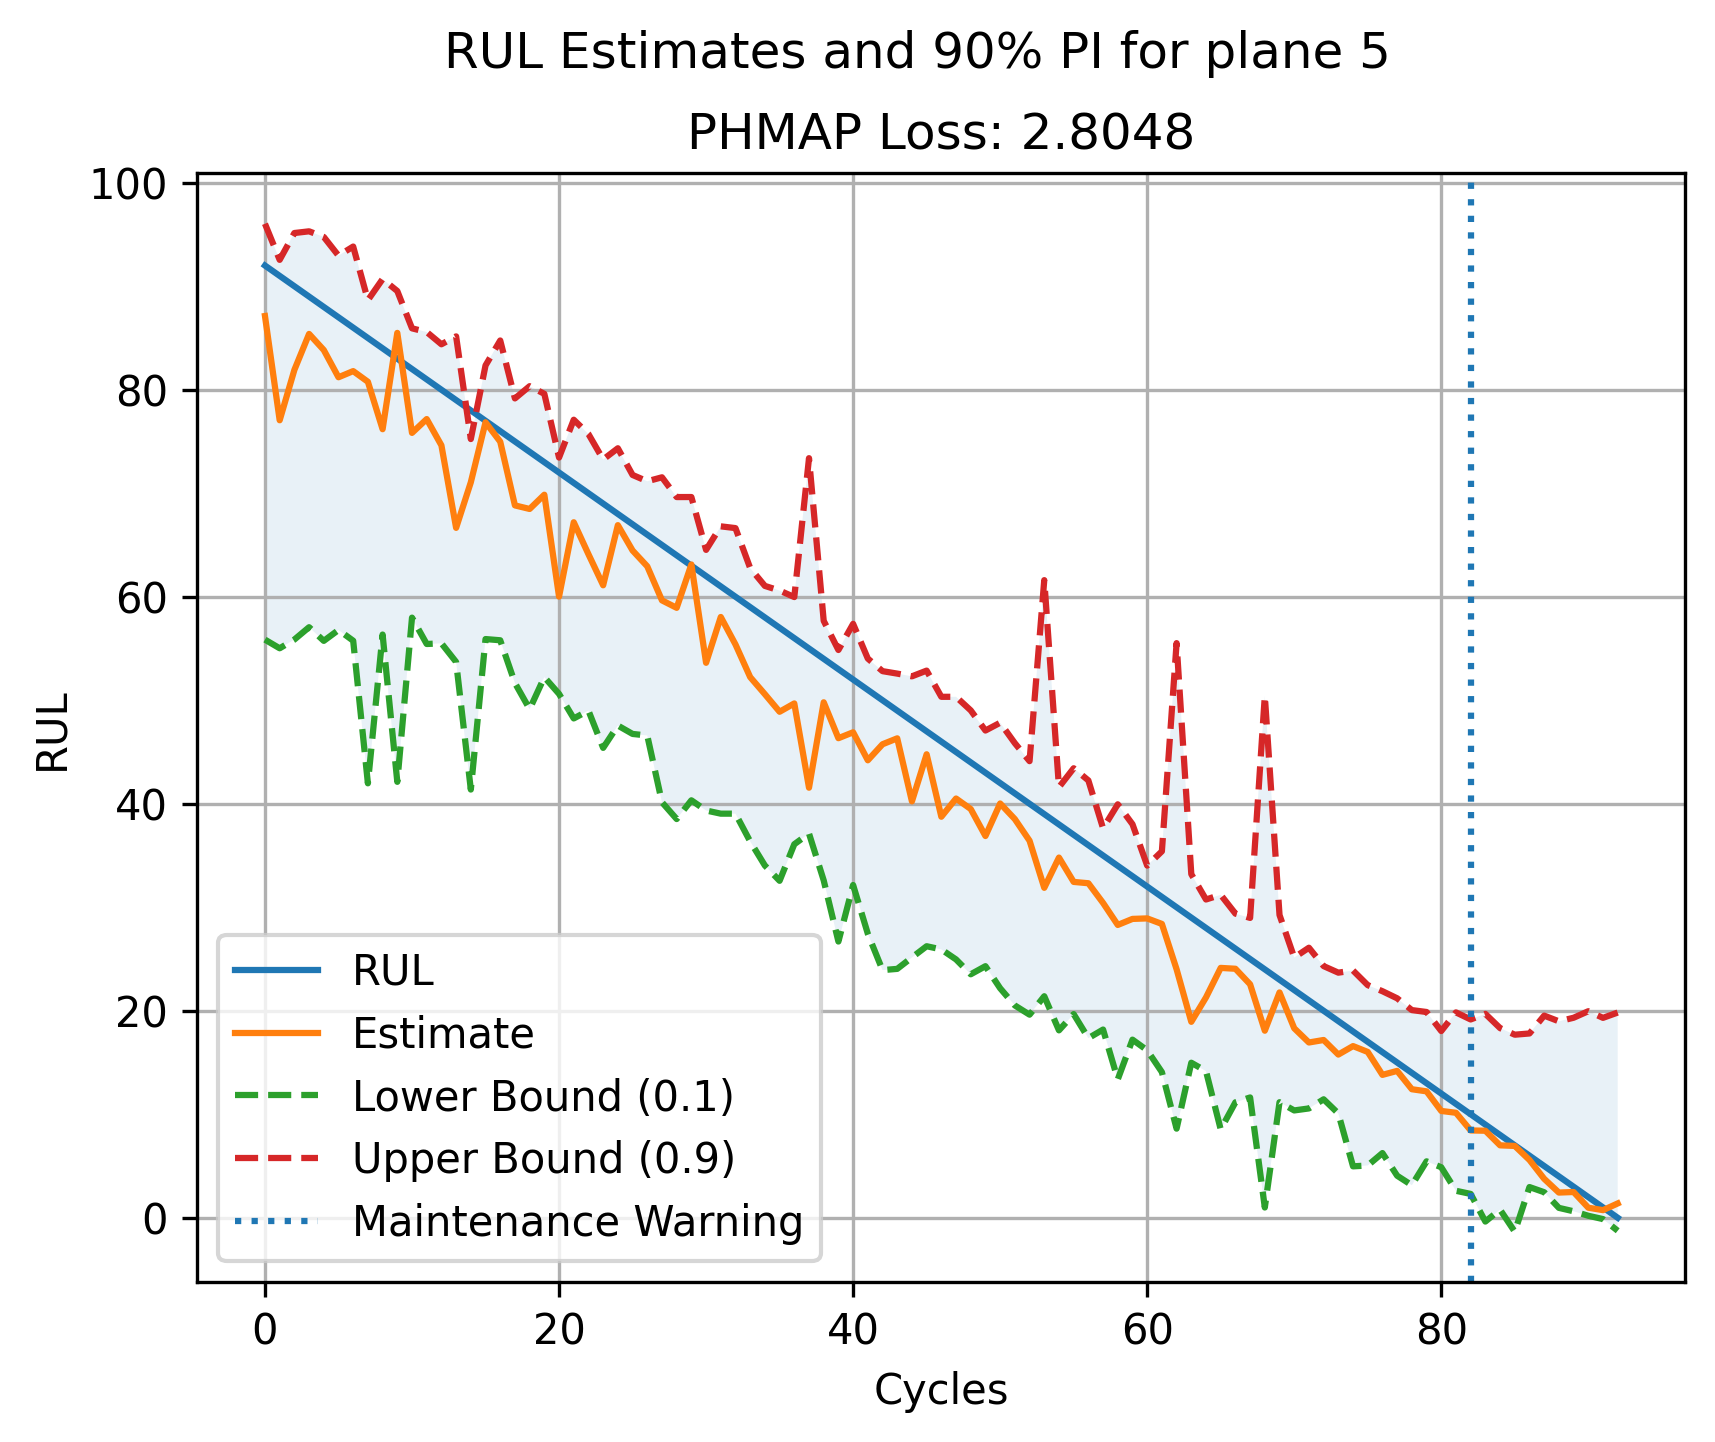
\includegraphics[scale=0.47]{preds_DS03-012_5.png}
                \caption{RUL estimates and PI for the operational life of a plane.}
                \label{fig:sample_estimates_pi}
            \end{figure}

            Notably, the model tends to adopt a conservative approach in its predictions, aligning with the intended effect of the PHMAP loss function, where a preference for underestimates is established for safety considerations. Additionally, the provided Prediction Interval (PI) offers stakeholders a relative measure of prediction uncertainty at each point. It is noteworthy that the PI tends to flatten towards the end of the plane's operational life, indicating that the conforming models have learned the general behavior of planes during this final stage. These observations collectively emphasize the reliability and safety-conscious nature of the RUL estimation model.

            To further enhance safety measures, the research suggests issuing a maintenance warning whenever the model predicts a Remaining Useful Life (RUL) value that falls below the Root Mean Square Error (RMSE) computed for the entire dataset.

            To offer a deeper insight into the predictions generated by the Remaining Useful Life (RUL) estimator, Shapley values were computed for each prediction of the dataset. Figure \ref{fig:shap_summary} presents the distribution of Shapley values for the top 12 features utilized by the model, ranked by the mean absolute Shapley value across the predictions.

            The color scale, transitioning from blue to red, signifies the relative values of features in terms of high or low, considering their distribution. On the x-axis, Shapley values are associated with each feature numerical value. For instance, the Shapley values affirm that as the flight number increases, the model predicts a lower Remaining Useful Life (RUL), as indicated by the high negative values for high flight numbers.
            \begin{figure}[H]
                \centering
                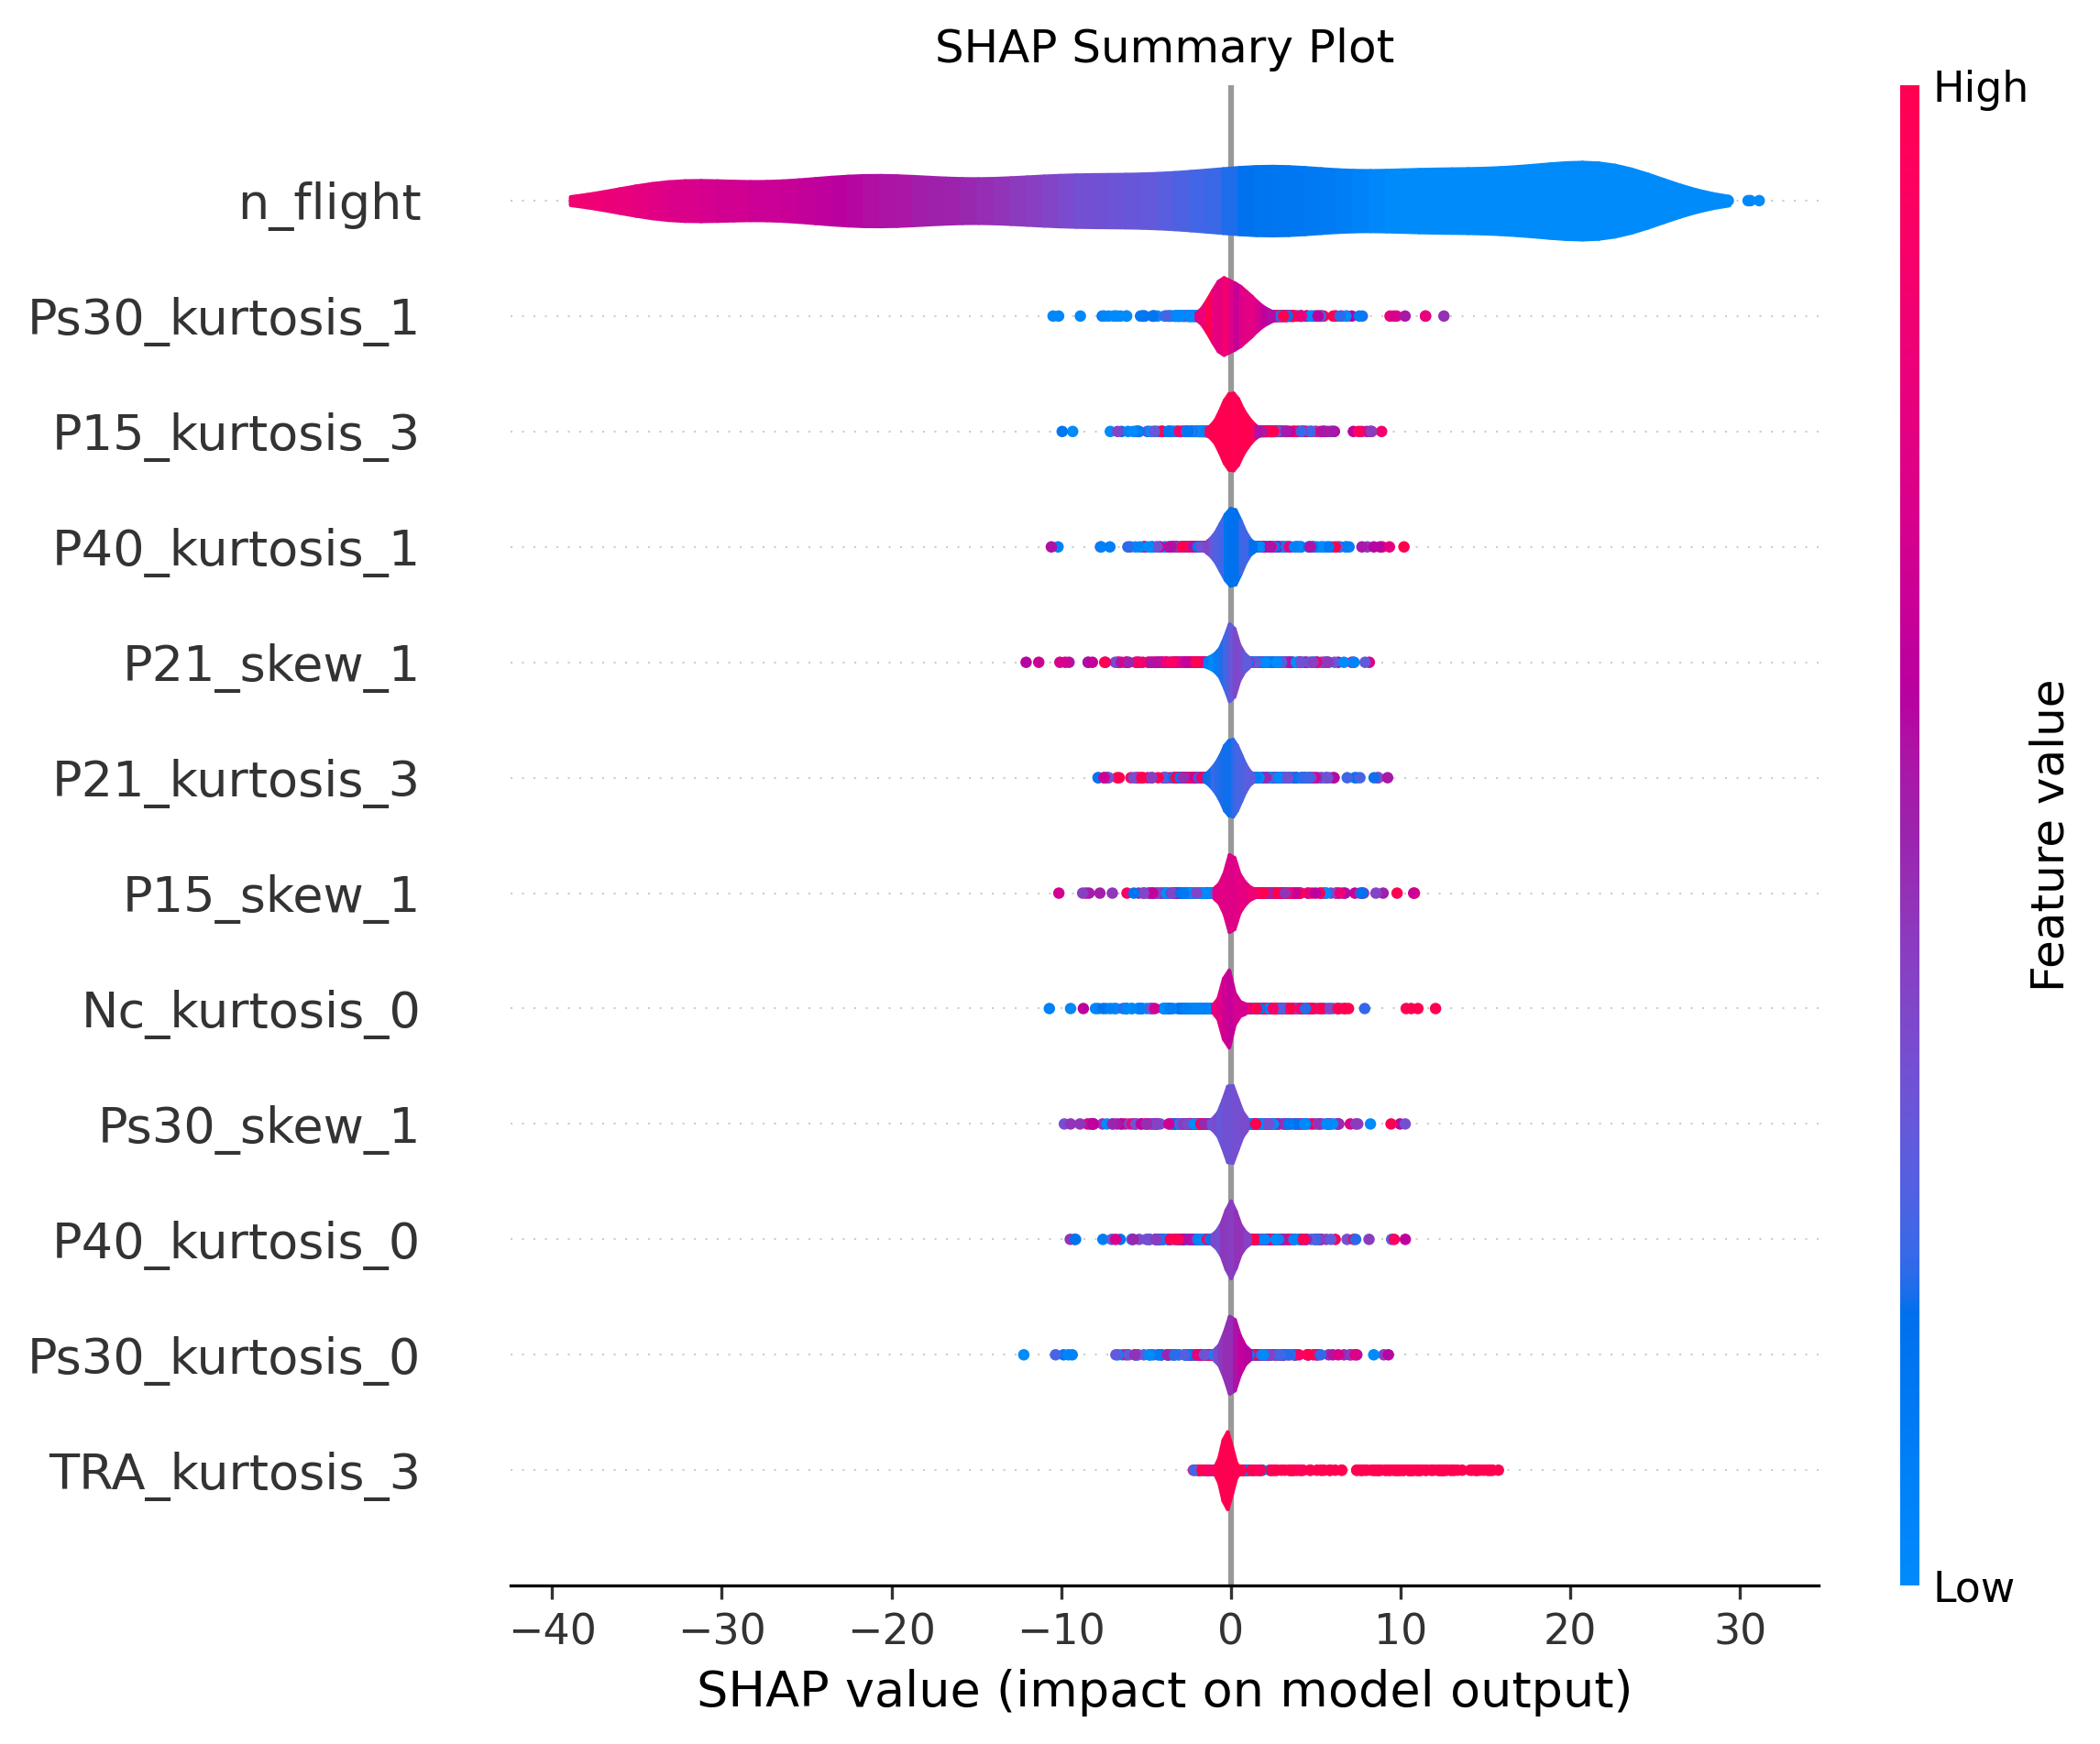
\includegraphics[scale=0.35]{shap_summary.png}
                \caption{Summary of Shapley values for the dataset.}
                \label{fig:shap_summary}
            \end{figure}

            For more detailed analysis, individual predictions can be examined, as shown in Figure \ref{fig:shap_instance}. This figure depicts how each feature value, accompanying each feature label on the left vertical axis, deviates the model predictions from their expected value (shown in the lower right corner) to the point where they add up to the actual prediction, labeled as $f(x)$, for this example in specific, the most important feature was the flight number, its Shapley value shows how being at its 57th flight reduces its operational cycles by almost 16 from the average prediction for all the planes in the dataset.
            \begin{figure}[H]
                \centering
                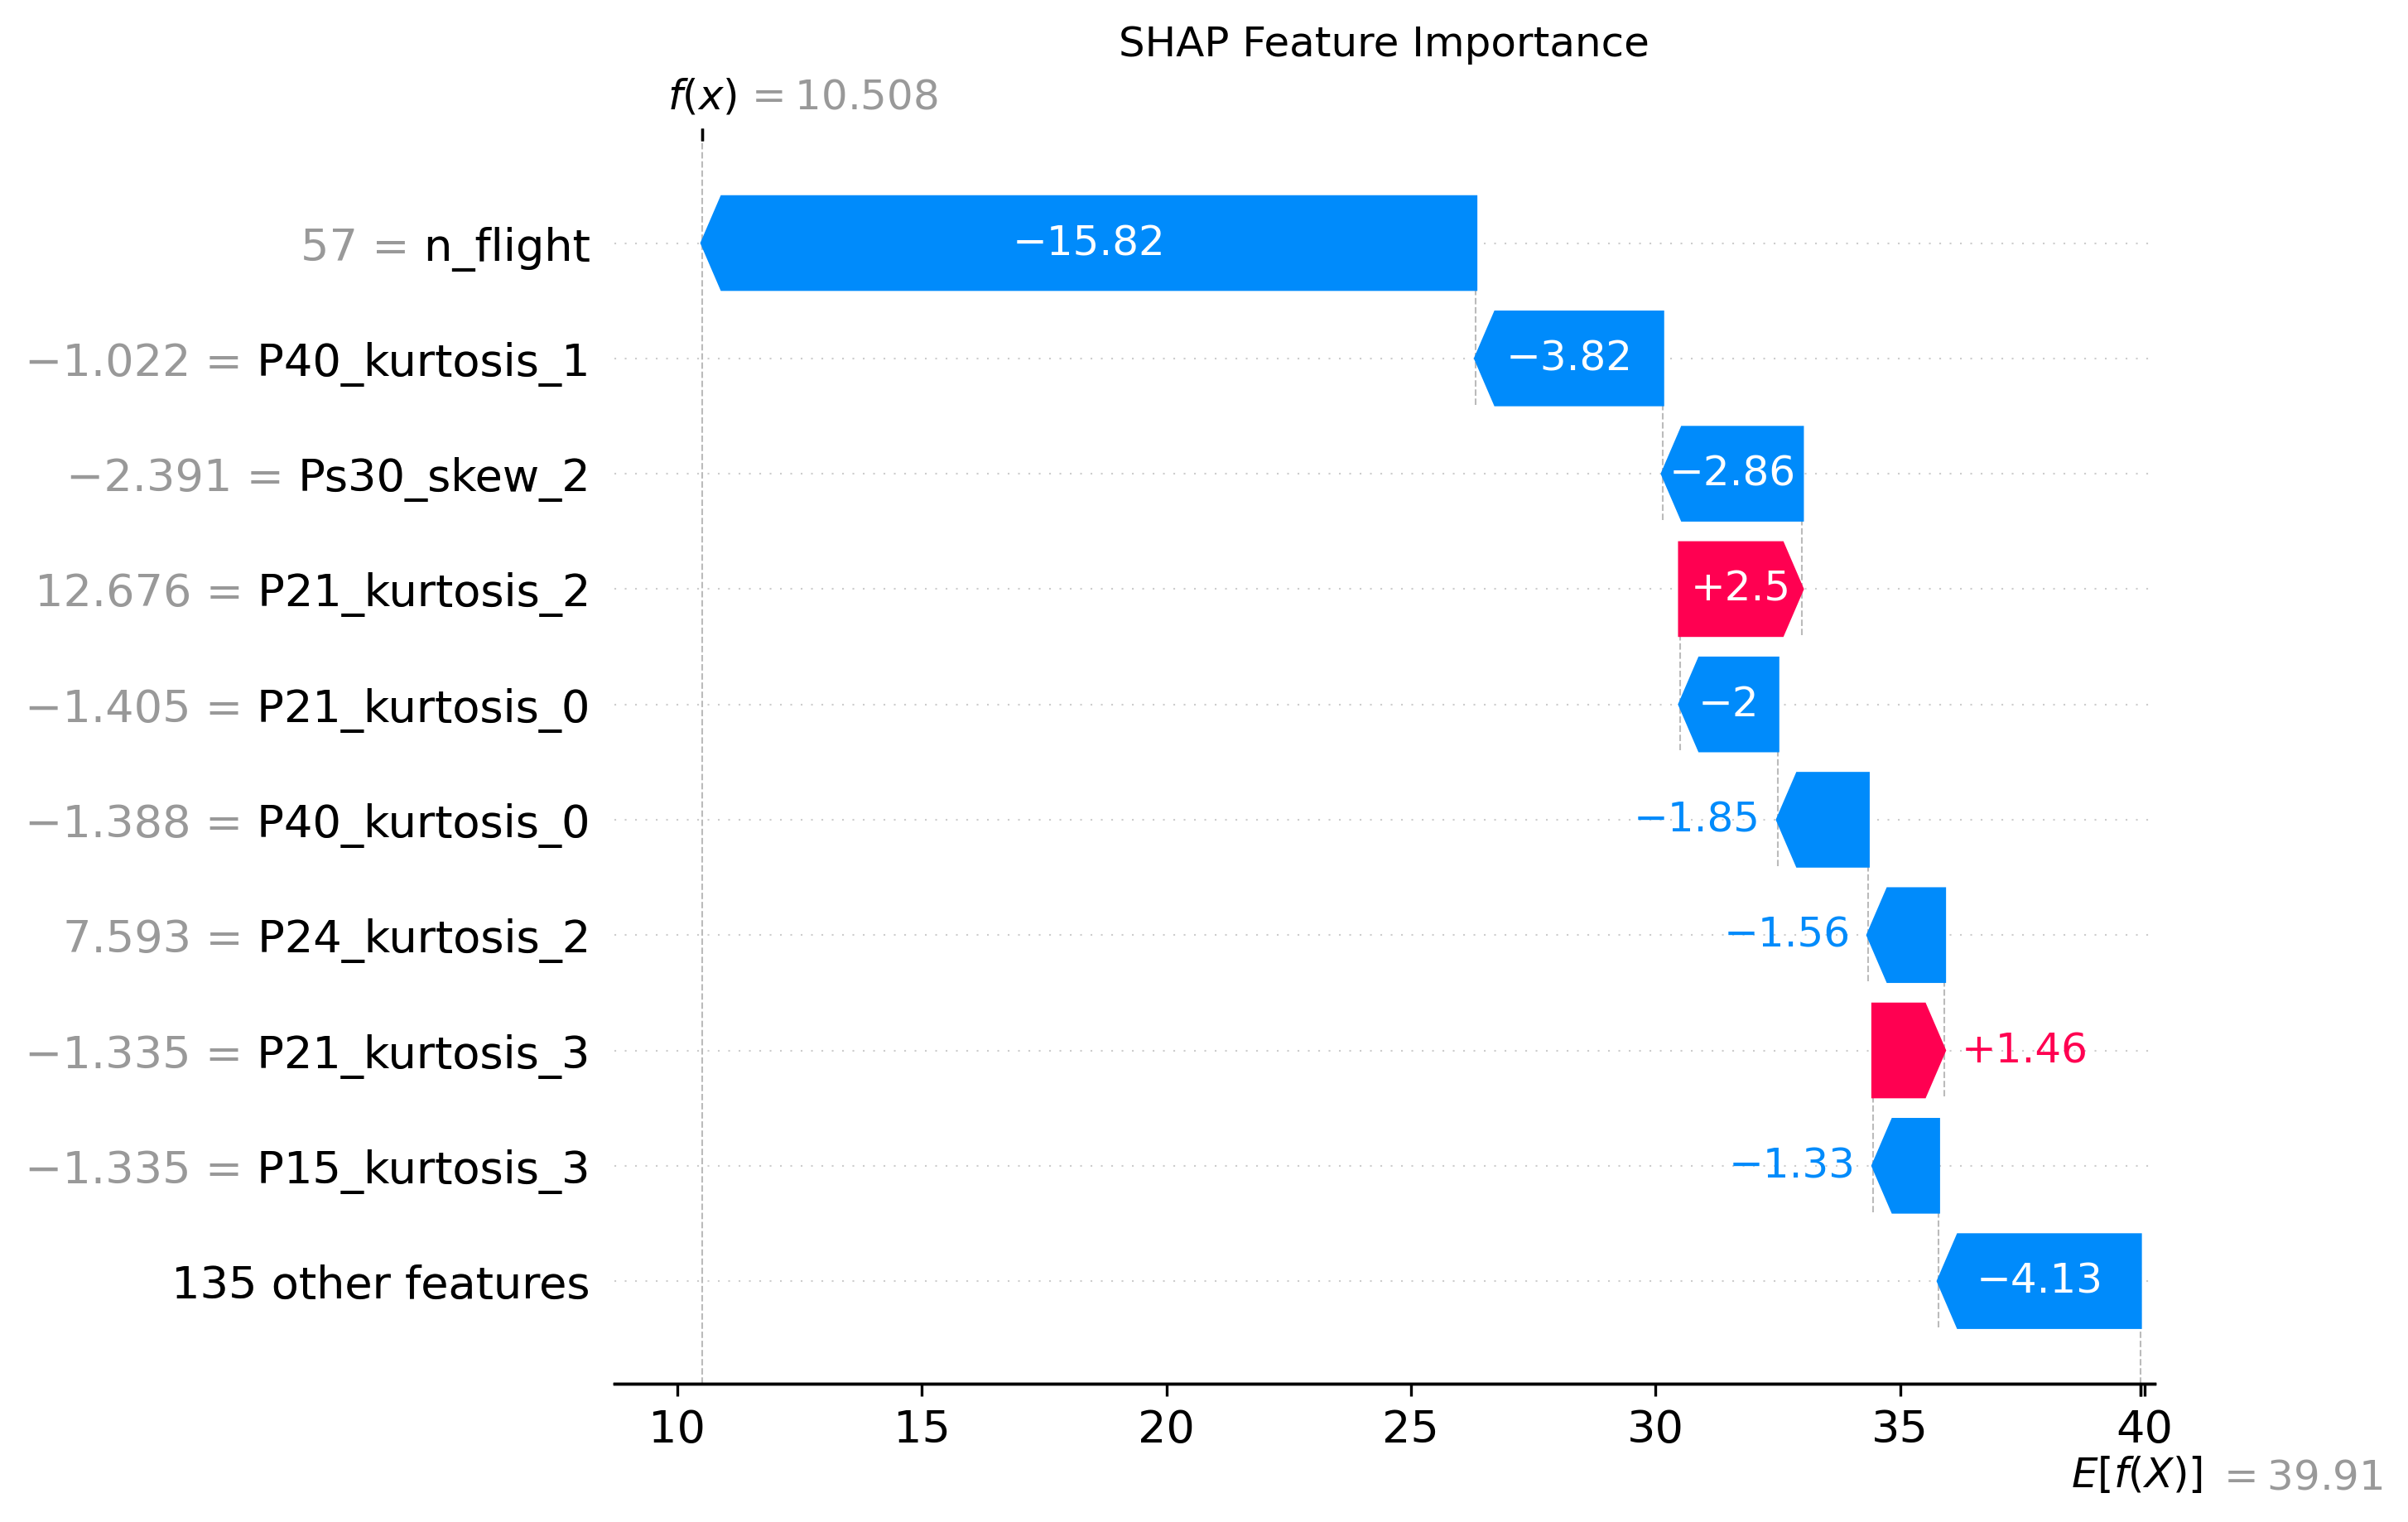
\includegraphics[scale=0.35]{shap_waterfall_example.png}
                \caption{Example of Shapley values for a single prediction.}
                \label{fig:shap_instance}
            \end{figure}

    \section{Conclusion and future work} \label{sec:conclusion}

        The research has yielded a comprehensive toolbox of techniques and utilities developed to optimize models systematically, resulting in improved performance beyond their basic counterparts. Although the models in this study provided predictions on a par with those achieved through Deep Learning methods, there was a slight reduction in overall performance \cite{phm-leaderboard}. The trade-off is best evaluated against the notable advantages offered by the models, including faster and more efficient training and inference processes and enhanced interpretability through the provided tools.

        Looking forward, potential future work encompasses the incorporation of the segmentation algorithm into the hyperparameter optimization process. This entails exploring various segmentation methods and determining the optimal number of segments, which may lead to further performance enhancements. This will increase the complexity of the process and will need a more robust error handling system.

        Another avenue for exploration involves modifying the feature selection technique by replacing the variance-based approach with the coefficient of variation. This adjustment could lead to more robust feature selection, particularly for features within a narrower range of values. Standardizing features by their mean can improve the model's capabilities.

        Additionally, further experimentation with the hyperparameter optimization process is advisable. Simple adjustments, such as increasing the number of trials conducted by the Tree-structured Parzen Estimators (TPE) and broadening the search space intervals, may reveal superior configurations that were previously overlooked.

        In pursuit of continuous improvement, ongoing research endeavors aim to enhance the effectiveness and efficiency of predictive maintenance frameworks, making a significant contribution to the evolving landscape of predictive maintenance methodologies.

    \bibliographystyle{IEEEtran}
    \bibliography{references.bib}
\end{document}